\documentclass[12pt,a4paper]{article}
\usepackage {amsmath,amsthm}
\usepackage{geometry}
\usepackage{titlesec}
 \geometry{a4paper, total={170mm,257mm}, left=20mm, right=20mm, top=25mm, bottom=25mm}
%\usepackage{tabularx}
\usepackage{sectsty}
\usepackage{natbib}
\bibliographystyle{econ}
\usepackage[hidelinks]{hyperref}
\usepackage{multirow}
\usepackage{makecell}
\usepackage{adjustbox}
\usepackage{ulem}
\usepackage{threeparttable}

%\usepackage[colorlinks=true, urlcolor=Blue]{hyperref}
%\usepackage{titling}
\sectionfont{\fontsize{14}{15}\selectfont}
\subsectionfont{\fontsize{13}{15}\selectfont}

\titleformat*{\section}{\LARGE\bfseries}
\titleformat*{\subsection}{\Large\bfseries}


\usepackage{caption}
\captionsetup{belowskip=12pt,aboveskip=0pt}

\makeatletter
\setlength{\@fptop}{0pt}
\makeatother


\usepackage[dvipsnames]{xcolor}

\newcommand{\link}[1]{{\color{blue}\href{#1}{#1}}}

%TRACKING TOOL FOR ARYA: 
\newcommand{\agt}[1]{{\color{OliveGreen}#1}}
\newcommand{\agst}[1]{{\color{OliveGreen}\sout{#1}}}

%TRACKING TOOL FOR ALEX: 
\newcommand{\aut}[1]{{\color{Red}#1}}
\newcommand{\aust}[1]{{\color{Red}\sout{#1}}}

%TRACKING TOOL FOR Peter: 
\newcommand{\pmt}[1]{{\color{Blue}#1}}
\newcommand{\pmst}[1]{{\color{Blue}\sout{#1}}}


%\usepackage{cite}
\usepackage{booktabs}
\usepackage{float}
\usepackage{setspace}
\usepackage{placeins}
\usepackage[list=true]{subcaption}
\captionsetup[sub]{font=footnotesize}

\usepackage{graphicx}


\newtheorem{theorem}{Proposition}
\newtheorem{hypothesis}{Hypothesis}
	\def\hypothesisautorefname{Hypothesis}
\newtheorem{result}{Result}
	\def\resultautorefname{Result}
\def\sym#1{\ifmmode^{#1}\else\(^{#1}\)\fi}


\title{\Large Crying Wolf in the Lab\\}
\author{\large Arya Gaduh, Peter McGee, Alexander Ugarov*}
\begin{document}
\maketitle
\onehalfspacing
\begin{abstract}{ Abstract is here ----}


\vspace{10pt}
\begin{singlespace}

\noindent {\footnotesize{}Keywords: alarms, value of information, information economics, information design, --- }{\thispagestyle{empty}}
\end{singlespace}
\end{abstract}

\vspace{180pt}
\newpage
\normalsize

\section{Introduction}

The 2010 gas blowout on Deep Horizon oil rig has killed 11 workers and caused one of the largest oil spills in history. The death toll was possibly aggravated by switching off a general safety alarm because its sirens interfered with workers' sleep.\footnote{https://www.nytimes.com/2010/07/24/us/24hearings.html} This illustrates the trade-off between false-positive and false-negative test results with false-positive rates leading to higher false alarm costs and false-negative resulting in missed events. 

Many real-life situations involve choosing binary tests to discover and prevent a negative outcome. Most binary tests transform continuous signals about the likelihood of an adverse state into simple yes/no prediction. This transformation relies on choosing a threshold for positive classification. Holding a continuous signal constant, a decrease in probability of no alarm in an adverse state (false-negative rate) corresponds to an increase in probability of alarm in a non-adverse state (false-positive rate). This trade-off motivates multiple discussions in medical diagnostics, alarm systems and extreme weather alerts. Despite ubiquity of binary alarms, there is little empirical evidence on how users evaluate alarms with different false-positive and false-negative rates. 

In order to understand preferences over these trade-offs, we study the demand for information in the framework with a potential protection action. The subject, first, receives a signal about the probability of an adverse event. Then she decides to protect or not. This environment describes several practically important scenarios including extreme weather alerts, medical testing and safety alarms. 

Some recent studies observe that many people put non-zero value on information about ego-relevant beliefs or future utility even if it has no apparent effect on subsequent decisions (all the citations). These preferences is not the focus of our study and hence we use relatively low stakes and ego-neutral information. As a result, our findings might not apply to settings with changing identity beliefs or to settings with delayed resolution of uncertainty and large potential payoffs. 

We find that the value of information in our setup weakly correlates with the willingness-to-pay. First, subjects on average underreact to quality of the signal, resulting in overpaying for low-quality signal and underpaying for high-quaity signals. Second, subjects tend to overreact to false-negative rates when the prior probability is low and overreact to false-positive positive rates when priors are high. We show that this pattern is most consistent with failure to estimate the effect of frequencies of false-positive and false-negative outcomes on the costs of using the signal. Xu (2020) similarly finds that individuals(?) do not properly account for priors and often choose tests not affecting optimal decisions even then more instrumental tests are available.

Our work is one of a few experimental studies measuring demand for information used for decision-making (instrumental information). Previous experimental studies studies the demand for signals in the prediction game in which subjects have to choose an optimal state under uncertainty. The field experiment conducted by \citep{hoffman_how_2016} finds that the demand for information increases with initial uncertainty, but decreases with the signal's accuracy. However, the decrease in accuracy is more modest than expected for a Bayesian decision-maker resulting in subjects underpaying for high-quality signals. The laboratory experiment of \citet{ambuehl_belief_2018} finds that subjects tend to underreact to the accuracy of the binary signal about state of the world, but put a premium on completely certain signals. The paper of \citet{xu_revealed_2020} similarly employs a prediction game but varies priors on top of signal charasteristics. reducing prior uncertainty makes more signals non-instrumental in the sense that there should be no effect from a signal to optimal decisions.  She find that many subjects choose non-instrumental over instrumental signals which is consistent with

Our setup differs in two important aspects from \citep*{ambuehl_belief_2018, xu_revealed_2020}, because we study alerts and not prediction tasks. The subject faces a costly protection decision and not a prediction decision, resulting in three distinct payoffs: full payoff, full payoff minus protection costs and full payoff minus losses. It means that risk preferences affect the value of information and can change sensitivities to false-positive and false-negative rates. Our findings however are similar to prediction game findings. Consistent with \citet{ambuehl_belief_2018} we also find that subjects undervalue accurate signals, but we do not find a premium for certain signals.  And similar to \citet{xu_revealed_2020} we find that subjects do not properly account for interaction between prior probabilities and signal characteristics.

Due to its applicability for studying preferences over expectations, there is a larger stream of literature on the demand for non-instrumental information. \citet{eliaz_paying_2010} find that subjects are willing to pay for signals even when these signals are excessive for making optimal choices. Their design involves subjects choosing between two boxes with one box containing a prize of \$20. Most subjects pay just to know the probability of finding \$20 in box A even if this box is more likely to contain a prize in all the possible states. This finding is inconsistent with expected utility maximization but indicates instead having preferences for certainty before making choices.  Similar to this paper, \citet{masatlioglu_intrinsic_2017} also study preferences over information structures differing which differ in false-positive and false-negative rates but in their setup allows for a larger role of expectations. They find that for a positive potential outcome, most subjects prefer facing high false-negative rates rather than high false-positive rates. In other words, they tolerate uncertainty after negative signals better than uncertainty after positive signals. These preferences are salient: subjects require an average payment of 18-35 cents to switch to their least preferred information structure.

There is some mixed evidence that people update beliefs differently when these beliefs are ego-relevant or concern future gains and losses. \citet{eil_good_2011} find asymmetry in updating ego-relevant beliefs such as beauty and IQ. Subjects update more after receiving positive signals and do not update enough after negative signals. Additionally, subjects with high posterior ego-relevant beliefs are willing to pay to receive a more precise signals, but require a compensation for learning when their beliefs are low. In contrast, \citet{coutts_good_2019} does not find any updating asymmetry with respect to either ego-relevant beliefs or beliefs about future payoffs. 

Our paper is the first to measure value of information in the experimental setting of diagnostic tests or alarms. Previous work studies the use of alarms in context of medical testing, medical monitoring, safety alarms and extreme weather. Early literature on decision-making of medical professionals finds that doctors suffer from multiple biases when ordering testing, including  inaccurate posterior probability estimation due to availability heuristics, hindsight bias and regret \citep{bornstein_rationality_2001}. \citet{gigerenzer_helping_2007}find that very few mammologists understand mamogram results and tend to overestimate probability of cancer based on a positive result. Providing practitioners with natural frequencies instead of probabilities tends to reduce this bias.  

Patients' willingness-to-pay for medical tests is large and largely responsive to test accuracy \citep{liang_acceptability_2003, howard_does_2009, neumann_willingness--pay_2012}. But there are several apparent violations of rationality. First, users are willing to pay for tests having little or zero diagnostic value \citep{schwartz_enthusiasm_2004, neumann_willingness--pay_2012}. For example, \citet{schwartz_enthusiasm_2004} find that 73\% of Americans in their survey prefer a free full-body CT scan versus one thousand USD cash. However, medical professional do not recommend full-body CT scans for healthy people due to extreme likelihood of false-positive findings. Second, the framing of test accuracy seems to matter a lot. \citet{howard_does_2009} conduct a discrete-choice experiment to measure willingness-to-pay for the colorectal cancer screening. Their subjects agree to get 23 unnecessary colonoscopies in order to find one additional true cancer, but only 10.4 for reducing the number of cancers missed by one even though these descriptions are equivalent. Surprisingly, the perceived risk of cancer (prior) did not significantly affect the WTP in their study though the effect may come from its relatively low variation in the population.

This work also relates to the vast literature on demand for insurance and protection. Similar to our findings, several studies observe that the demand for insurance goes up after the recent experience with low-probabiity events. Field evidence indicates that people underinsure with respect to rare natural disasters (Friedl et al, 2014). \citet{laury_insurance_2009} find no under-insurance for low-probability events in the laboratory setting. One offered explanation \citep{volkman-wise_representativeness_2015} is that subjects overweight recent evidence leading to underinsurance when there were no negative events in the recent past and to overinsurance after the fact. It is consistent with underweighting prior probabilities relative to more recent signals. 

The bias we are finding is similar to the base-rate and signal neglect phenomenons. Psychology researchers \citet{hammerton_case_1973} and \citet{kahneman_psychology_1973} first observed that subjects underweighted prior probabilities (base rates) when calculating posteriors. This phenomenon had received the name of \textit{base-rate neglect}. Multiple studies in economics then confirmed \citep*{grether_testing_1992, holt_update_2009} this phenomenon in incentivized laboratory experiments. Most of these studies find that subjects also underweight signals on top of priors.  We observe both phenomenons in responses to our belief elicitation task, but the calculation of signals' values differs substantially from the calculation of posterior probabilities. While the calculation of posterior probabilities would require using a Bayes formula, signal's value depends only on products of prior probabilities. However, we observe that subjects underestimate the effect of priors compared to theoretical predictions for an expected-utility decision-maker.


\vspace{20pt}

\section{Model}
\vspace{10pt}
\bf Environment. \rm The model describes a decision-maker considering a purchase of threat-assessment information. Let $\omega \in \{0,1\}$ denote the state of world, where 1 corresponds to some adverse event happening with probability $\pi$. The decision-maker has a lower utility in the adverse state, but only if she does not take the protective action. Denote actions by $a\in\{0,1\}$ with 1 meaning taking the protective action. The protection technology is perfect: protected agents bear no losses but pay protection costs $c$ regardless of the state $\omega$. Decision-maker preferences are described by the utility function which depends on wealth $Y$, protective action $a$ and potential damage in the adverse state $\omega(1-a)$. Utility is separable in wealth, protection costs $c>0$ and potential loss in the adverse state $L>c$ \footnote{Separability condition does not impose additional restrictions on the utility function $U$ as long as the variation in wealth has limited range. More specifically, if $Y \in [Y_{min},Y_{max}]$ and $c<Y_{max}-Y_{min}, L<c+(Y_{max}-Y_{min})$, then the function $u(\cdot)$ can be constructed from segments of $U(\cdot,0,0), U(\cdot,1,0), U(\cdot,0,1)$.  While the resulting function $u(\cdot)$ is not necessarily monotonic, it is likely to be monotonic if protective actions and potential damages are relatively high.}:
\begin{equation}
U=U(Y,a,\omega(1-a))=u(Y-ac-\omega(1-a)L)
\end{equation}

The decision-maker can purchase a binary informative signal $s\in\{0,1\}$ about the state of the world before making a decision. Let $P_{ij}\equiv P(s=i|\omega=j)$ be the probability of a signal taking value $i$ conditional on the state of the world being $j$.  After receiving the signal, the decision-maker updates her belief on the likelihood of the bad state to $\mu(s)$. Unless specified otherwise, we assume that the decision-maker forms her posterior beliefs by using the Bayes rule. Hence the posterior belief equals:
\begin{equation}
\mu(s)= {\pi P_{s1} \over \pi P_{s1}+(1-\pi)P_{s0}}
\end{equation}

We also assume without loss of generality that a higher signal means a higher posterior probability of an adverse event $\mu(1)\geq\mu(0)$. Otherwise we can always re-label the signals.

\vspace{10pt}
\bf Preferences. \rm If there is no signal, the decision-maker protects if and only if it increases their expected utility:
\begin{equation}
EU_0=\max[u(Y-c),\pi u(Y-L)+(1-\pi) u(Y)]
\end{equation}
The signal can increase expected utility if the decision-maker reacts differently to positive and negative signals. Under these assumptions, her expected utility with a signal is:
\begin{equation}
EU_s=\pi P_{11}u(Y-c)+\pi P_{01}u(Y-L)+(1-\pi)P_{10}u(Y-c)+(1-\pi)P_{00}u(Y)
\end{equation}

We consider the maximum amount $b$ which the decision-maker is willing to pay for the signal. In our framework, it is a price paid with a signal such that a decision-maker is indifferent between having a signal and paying $b$ and not having a signal. Because the decision-maker can always ignore a useless signal, the signal's value is bounded from below by zero. Hence it equals to the maximum between zero and the solution to the following equation:
\begin{equation}
\begin{split}
P(s=1)u(Y-b-c)+\pi P_{01}u(Y-b-L)+(1-\pi)P_{00}u(Y-b)=\\=\max[u(Y-c),\pi u(Y-L)+(1-\pi) u(Y)] 
\end{split}
\end{equation}

The left-hand side expression of this equation is a strictly decreasing function of $b$. Additionally, for $b\rightarrow \infty$ the left-hand side is smaller than the right-hand side. It implies that the equation (5) above has a at most one positive solution.

Obviously, perfectly accurate signals always have positive value $b>0$ because the payoff distribution with the signal first-order stochastically dominates the distribution without the signal. If the decision-maker protects without a signal, a perfect signal reduces the protection costs and if she takes chances, then it reduces losses in the adverse outcome from $L$ to $c<L$.  However, it is harder to determine the value of the imperfect signal without imposing more restrictions on preferences as it requires weighing $u(Y-L)$ against $u(Y-c)$.


\vspace{10pt}
\bf Risk-neutral agent. \rm If the decision-maker is risk-neutral, the expression above collapses to:
$$b+P(s=1)c+\pi P_{01}L=\min[c,\pi L]$$

The signal's value is just:
\begin{equation}
b=\max[0,\min[c,\pi L]-P(s=1)c-\pi P_{01}L]
\end{equation}

We can express WTP $b$ as a function of priors, false-positive and false-negative rates. This is the equation we use in our empirical work:
\begin{equation}
b=\max[0,\min[c,\pi L]-\pi (1-P_{01})c-(1-\pi)P_{10}c-\pi P_{01}L]
\end{equation}

The sensitivity of (positive) value $b$ with respect to false-positive and false-negative rates is given by:
\begin{equation}
{db\over dP_{10}}=-(1-\pi)c
\end{equation}

\begin{equation}
{db\over dP_{10}}=-\pi(L-c)
\end{equation}
\vspace{10pt}

Both false-positive and false-negative rates decrease the (positive) signal's value. The effect is proportional to the adverse state probability for the false-negative rate and to the non-adverse state probability for the false-positive rates.

\vspace{10pt}
\bf Risk Aversion Effects. \rm In a more general expected utility framework, risk aversion can both increase and decrease the signal's value. More specifically, risk aversion decreases the value when the protection costs are low: 

\begin{theorem}
 If protection costs are low $c<\pi L$, then the strictly risk-averse decision-maker pays less than a risk-neutral one.
\end{theorem} 
\begin{proof}
See the Appendix.
\end{proof}
It is harder to make definite statements for lower risks or higher protection costs. For example, risk aversion increases value of a perfect signal as long as risk-averse decision-maker still chooses to not protect without a signal. This follows from the standard argument of increasing demand for insurance with risk aversion and the fact that the protection problem with a perfect signal is isomorphic to the insurance problem with deductible $c$. 

Next, we study the effect of false-positive and false-negative rates on the signal's value $b$. Assuming a differentiable utility function $u()$ we use implicit differentiation to derive sensitivities of WTP $b$ to false-positive and false-negative rates:

$${db\over dP_{10}}=-{(1-\pi)(u(Y-b)-u(Y-c-b))\over D(\pi, P_{01}, P_{10}, b)}$$
$${db\over dP_{01}}=-{\pi(u(Y-c-b)-u(Y-L-b))\over D(\pi, P_{01}, P_{10}, b)}$$

With the denominator equal to the expected marginal utility:
$$D(\pi, P_{01}, P_{10}, b)\equiv P(S=1)u'(Y-c-b)+\pi P_{01}u'(Y-L-b)+$$
$$+(1-\pi)P_{00}u'(Y-b)=E[MU]>0$$

It is clear that the signal's value decreases with false-positive and false-negative rates ${db\over dP_{10}},{db\over dP_{01}}<0$. We can also say a bit more about the sensitivity to false-negative rates:
\begin{theorem}
Risk-averse and imprudent decision-maker has higher sensitivity to false-negative rates as compared to a risk-neutral one.
\end{theorem} 
\begin{proof}
Use the mean value theorem to rewrite the sensitivity as:
$${db\over dP_{01}}=-{\pi u'(\zeta)(L-c)\over E[MU]},\zeta \in \left(Y-c-b, Y-L-b\right)$$
Now let $X$ denote a random payoff of the decision-maker with a signal. A risk-averse decision-maker puts a positive value on the signal only if its expected payoff is higher than the payoff with full protection: $EX>Y-c-b$. If a decision-maker is imprudent ($u'''<0$) then $E[MU]\equiv E[u'(X)]<u'(EX)$. Next, because $u'$ is a strictly increasing function and $EX>Y-c-b$: $u'(\zeta)>u'(Y-c-b)>u'(EX)$. Hence ${u'(\zeta)\over E[MU]}>1$ and ${db\over dP_{01}}<-\pi(L-c)$. 
\end{proof}


However, risk aversion can both increase and decrease subject's sensitivity to false-positive rates depending on the utility function curvature and signal's characteristics. Intuitively, an expected marginal utility of a strongly risk-averse subject with a bad signal can be lower than the average slope of the utility function between $Y-c-b$ and $Y-b$ reducing sensitivity to false-positive rates. It can also be higher if either the signal is good or the curvature is small. 

\vspace{20pt}

\section{Experimental Design}

In each session, subjects received a USD 5 show-up fee and were endowed with USD 25 that they might lose in the experiment. Subjects must then make a series of decisions in four sets of tasks: (i) Blind Protection; (ii) Informed Protection; (iii) Belief Elicitation; and (iv) Willingness to Pay Elicitation. To verify that subjects understand these tasks, they must answer a quiz before each task. If a subject gets any answer wrong, they read correct answers and explanations for each wrong answer. Additionally, subjects receive extra questions if they give wrong answers in a 5-question quiz given before the Informed Protection task. We do this because we consider Informed Protection as a first challenging task in the sequence which understanding is essential for the rest of the tasks. 
Each set of tasks has 6 rounds, for a total of 24 rounds. One of these rounds is selected at random as the payment round. A copy of the instruction is included in Appendix XX.

\bigskip
\noindent\textbf{Blind Protection (BP)}.\ \ \ In each BP round, subjects must decide whether to insure (or “protect”) against an adverse event (i.e., drawing a black ball from a box).  Subjects were informed of the prior probability of drawing a black ball before making their decision. The cost to protect is USD 5. If a black ball is drawn, an unprotected subject will lose USD 20. Subjects then played six rounds, where the probability of drawing a black ball was varied between XX and XX percent in each round. During the BP task, subjects did not receive any feedback on how that round would have been realized were it chosen as the payment round.

\bigskip
\noindent\textbf{Informed Protection (IP)}.\ \ \ For the IP task, subjects make a protection decision as in BP. However, before each decision, subjects are given a signal that was generated with varying degrees of inaccuracy. Following Coutts (2019), we present the signal-generation process using groups of ``gremlins'' that represent three types of signals: accurate (an honest gremlin), false positive (a black-swamp gremlin that always announces that the ball is black), and false negative (a white-swamp gremlin that always announces that the ball is white). Figure XX illustrates how the different gremlin types were presented to the subjects. Subjects knew the composition of the group from which the hint came from, but did not know which gremlin provided the hint. We vary the proportion of black balls in the box (prior probability of a black ball) and the composition of gremlins (signal quality) between rounds.  

\bigskip
\noindent\textbf{Belief Elicitation (BE)}.\ \ \ We use the BE task to elicit subjects’ beliefs about the likelihood of an adverse event and an adverse signal conditional on prior and signal characteristics in an incentive-compatible way. Similar to the IP task, subjects were informed of the prior probability of a black ball and the composition of the group of gremlins that would provide an additional signal. However, instead of asking subjects to make a protection decision, we asked them to estimate the probability of two events, to wit: (i) the ball is black ball when a randomly drawn gremlin says that it is white; (ii) the ball is black when a randomly drawn gremlin says that it is black.   

We follow the stochastic version of the Becker-DeGroot-Marshak mechanism developed by \citet{grether_testing_1992} and \citet{holt_update_2009} to elicit incentive-compatible responses: the subject submits their belief of the probability of the event $\mu \in [0,1]$. If this belief is above some uniform random number $r\in[0,1]$, they receive the payoff $x$ only if the stated event happens. Otherwise their payoff is determined by an independent lottery which pays $x$ with probability $r$ and 0 otherwise.\footnote{The benefit of this mechanism versus other probability elicitation mechanism (for example, quadratic scoring) is that reporting truthfully is a dominant strategy regardless of risk preferences \citep{karni_mechanism_2009-1}. The only requirements a subject needs to satisfy are probabilistic sophistication and dominance: they rank lotteries based on their probabilities only and prefer higher probabilities of higher payoffs.} To help subjects understand this complex mechanism, we prefaced our explanation of it with the fact that under this mechanism, truthful reporting of beliefs is the dominant strategy.

\bigskip
\noindent\textbf{Willingness to Pay Elicitation (WTPE)}.\ \ \ The WTPE task measures subjects' willingness to pay (WTP) for signals. Subjects know the prior probability of a black ball and the group composition of the gremlins that will determine signal quality.  We then ask subjects for their WTP to receive a hint from a randomly drawn gremlin. Subjects can choose a value from USD 0 to 5 with USD 50-cent increments. Their decisions are incentive compatible: if a WTPE round is selected as the payment round, a random price of a hint will be drawn. If that price exceeded the subjects’ WTP, they will play a BP round. Otherwise, the subject would pay for the hint and play an IP round.  After completing the WTPE task, subjects were asked a few demographic questions. The session concluded with the random selection and realization of the payment round, after which subjects were paid and dismissed.

The first three tasks were designed to provide measures of the different components of WTP described in Section XX and use them to examine the extent to which they explain subjects’ WTP measured in the WTPE task. We use the BP task both to measure subjects’ responses to the prior and their risk aversion. Next, we use the IP task to examine how signals affect protection decisions. Finally, we use the BE task as a measure of subjects’ ability to estimate the probability of a signal for a given quality and to perform Bayesian updating. To construct these measures, we presented our subjects with 6 different priors for the BP task, and 3 priors and 2 gremlin groupings for the IP, BE, and WTPE tasks. Table~ref{tab:treatments} XX shows the values of the different priors in our treatments, as well as the gremlin groupings (along with the associated false positive and false positive rates) that we used for the different tasks.

We conducted this experiment in the Behavioral Business Research Lab (BBRL) at the University of Arkansas between October and November 2021.  The experiment was implemented using Qualtrics. There were a total of 105 subjects. 84 percent of the subjects were university students and 41 percent were male.  About 60 percent of the subjects had taken at least one statistics course. On average, including the show-up fee, subjects received around USD 26 for a session lasting around 45 minutes.  



%%%%%%%%%%%%%%%%%%%%%%%%%%%%%%%%%%%%%%%%%%%%%%%%%%%%%%%%%%%%%%%%%%%%%%%%%%%%%%%%%%%%%%%%%%%%%%%%%%%%%%%%
\pmt{I think we need to have panels for parameter values in BP to help understand BP in Fig.1}
\begin{table}[h!]
\caption{List of Treatments} \label{tab:treatments}
\begin{tabular}{l*{6}{c}}
\hline\hline
 & \multicolumn{3}{c} {Gremlins composition} & & \\
Prop. of black balls ($p$) & Honest & Black-eyed &White-eyed & FP rate &  FN rate\\
\hline
0.1, 0.2, 0.3, 0.5         &    2 & 0  &  0 & 0 & 0\\

0.1, 0.2, 0.3, 0.5         &    3 & 1  &  0 & 0.33 & 0  \\

0.1, 0.2, 0.3, 0.5          &    3 & 0  &  1 & 0 & 0.33 \\

0.1, 0.2, 0.3, 0.5           &    3 & 1  & 1 & 0.33 & 0.33\\

0.1, 0.2, 0.3, 0.5         &    5 & 1  & 0 & 0.2 & 0\\
0.1, 0.2, 0.3, 0.5         &    5 & 0  & 1 & 0 & 0.2    \\
0.1, 0.2, 0.3, 0.5         &    5 & 1 & 1  & 0.2 & 0.2  \\
\hline\hline
\end{tabular}


\end{table}

%%%%%%%%%%%%%%%%%%%%%%%%%%%%%%%%%%%%%%%%%%%%%%%%%%%%%%%%%%%%%%%%%%%%%%%%%%%%%%%%%%%%%%%%%%%%%%%%%%%%%%%%






\vspace{20pt}
\section{Results}\label{sec:results}
\pmt{I'm not going to futz with the sections right now, but I would make section 4 Subject Decisions, then have various subsections}
\pmst{We begin with a brief overview of subject behavior in the different tasks. }

%XXXX NEED TO REWRITE HERE XXXX}

Overall, we find that subject behavior across our tasks is largely ``sensible," i.e., subjects respond to increases in risk by protecting more, but deviates from the risk-neutral theoretical benchmark.  Below we investigate several standard possible explanations, including risk preferences and failures of Bayesian updating, before exploring how the characteristics of the signal influences protection decisions, beliefs, and WTP.

We follow that discussion with a regression analysis to explain subjects’ WTP for signals of different qualities. Our regression results suggest that subjects’ WTP deviated from those of a risk-neutral utility maximizing subject which was driven by their failure to fully account for signal quality when calculating their WTP. Furthermore, we find that these deviations remained after controlling for risk aversion or subjects’ ability to perform Bayesian updating. 

%The final subsection explored theories that are consistent with these observed behaviors.



%\subsection{Overview: Are Subjects Bounded Rational?}
\subsection{Blind Protection}



\pmst{\textbf{Blind Protection.}}\pmst{Subjects’ responses in the BP task are generally consistent with the expected utility framework.} Figure~\ref{fig:ProtResponse} plots the probability of protection decision against \pmst{prior}posterior probability of a black ball for the BP task, where the posterior is equivalent to the prior, and the IP task. On aggregate, subjects protect more with a higher probability of a negative outcome: only 13\% subjects protect when the probability of a black ball is 10\% in contrast to 70\% protecting when the probability is 30\%. 
%Moreover, the majority of subjects (54\%) have a probability threshold above which they always protect. About 30\% of subjects make at least one switch in which they protect for probability $P_1$ and do not protect for at least one probability $P_2>P_1$. 

At the individual level, BP responses are also largely sensible but  indicate significant heterogeneity in terms of risk aversion. For approximately 70\% of subjects (X/Y), the probability of choosing protection increases monotonically in posterior probability. The remaining 30\% make at least one switch from protecting to not protecting and back, which is inconsistent with EU maximization. Among these switchers, however, 83\% (24/39) skip only a single increment of the presented probability scale, suggesting an inattention error.\footnote{For comparison, this reference on the Holt and Laury (2002) instrument suggests the XX\% (YY\%) of subjects switch at least (at most) once.}  Risk-neutral subjects maximize their expected utility by protecting whenever the prior probability exceeds 0.25, which is the ratio of the protection cost (\$5) to the potential loss (\$20). In contrast, many of our subjects start protecting for lower probabilities of 0.1 or 0.2 indicating strict risk aversion. As a point of reference, switching at the probability 0.1 corresponds to CRRA risk aversion of $\theta=2$, while switching at 0.2 corresponds to $\theta=0.573$ (see \ref{ra_table} in Appendix).  \aut{I need to review the literature here to compare.} A smaller group of subjects makes choices consistent with risk loving by never protecting or protecting for the probability of 0.3. We use the total number of protection choices as a measure of subjects’ risk aversion, but following Holt and Laury (2002) exclude subjects switching more than once. Most of our results do not condition on risk aversion and hence are not affected by this calculation. \pmt{I don't understand exactly what you mean by using the total to ``calculate" risk preferences.  In HL, the total corresponds to a range for the parameter of a CRRA utility function, but I think we are just using the total as a relative metric in our sample?  Also, we probably need to make sure that everything doesn't go totally bananas if we include the multiple switchers, then offer in a footnote to send those results to anyone who cares.}

\subsection{Informed Protection}
%\bigskip\noindent\textbf{Informed Protection/Response to Signal.}\ \ \
Protection decisions are also positively correlated across tasks for a given individual.
Subjects receive more information in the IP task than in the BP task, though using that information requires that subjects engage in Bayesian updating.  Figure~\ref{fig:ProtResponse} shows that, consistent with their behavior in the BP task, the share of subjects protecting in the IP task is increasing in the posterior probabilities. More subjects display non-monotonic response to posterior probability of a black ball or, in other words, they do not protect for some  treatments with posterior probability $P$ while protecting for a posterior probabilty $P'<P$.  is higher than the probility of those they  switch back to no protection when Behavior is noisier, likely due to the fact that subjects have to calculate the posterior.\pmt{I'm not sure what we mean by ``noisier" here.  Is it more overall switching?  Within individual inconsistencies?  Greater discrepancies between posteriors at which they switch?}  At the individual level, we also observe a that the total number of times subject choose protection in the BP task significantly correlates with their likelihood to protect in the IP task conditional on posteriors, but explains only a very small part (<1\%) of variation in the IP decisions\footnote{We use a LPM to estimate this relationship, and while the coefficient on the total number of protection choices is significant at 99\%, $R^2$ increases from 0.295 to 0.3.} \pmt{I presume we have more inconsistent decision makers here?  It's worth putting a number to that, too, as we did for BP.  Are inconsistent BP guys more likely to be inconsistent here? }

Subjects' responses in the first two tasks suggest that conditional on the true probabilities, subjects protected more in the IP task compared to the BP task at low probabilities, \aut{even though the difference is not statistically significant}\pmt{What is the test? Proportion of protection decisions for probabilities less than X or something?}. These choices suggest that subjects’ updated beliefs overshot the true posterior at low probabilities.  Unfortunately, we cannot compare their decisions for higher probabilities because we do not present choices with higher prior in the BP task. \pmst{Do we want to bring up ambiguity aversion?  Do we discuss it again anywhere?  If not, it's probably better just to leave it out.}


%%%%%%%%%%%%%%%%%%%%%%%%%%%%%%%%%%%%%%%%%%%%%%%%%%%%%%%%%%%%%%%%%%%%%%%%%%%%%%%%%%%%%%%%%%%%%%%%%%%%%%%%%%%%%%%%%%%

\begin{figure}[H]
\centering
\caption{Average Protection Response} \label{fig:ProtResponse}
\begin{subfigure}[t]{.75\textwidth}
  \centering
  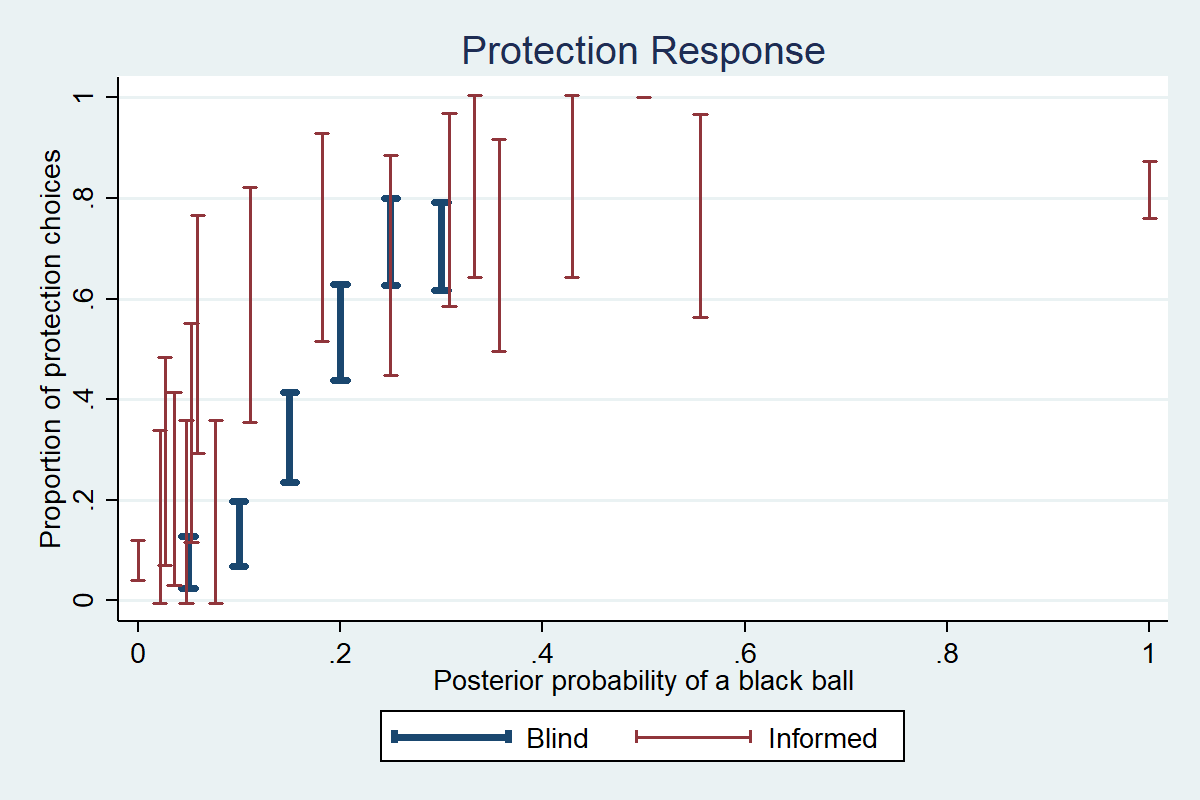
\includegraphics[width=\textwidth]{Graphs/ip_response_comp.png}
\end{subfigure}
%\begin{subfigure}[t]{.48\textwidth}
  %\centering
  %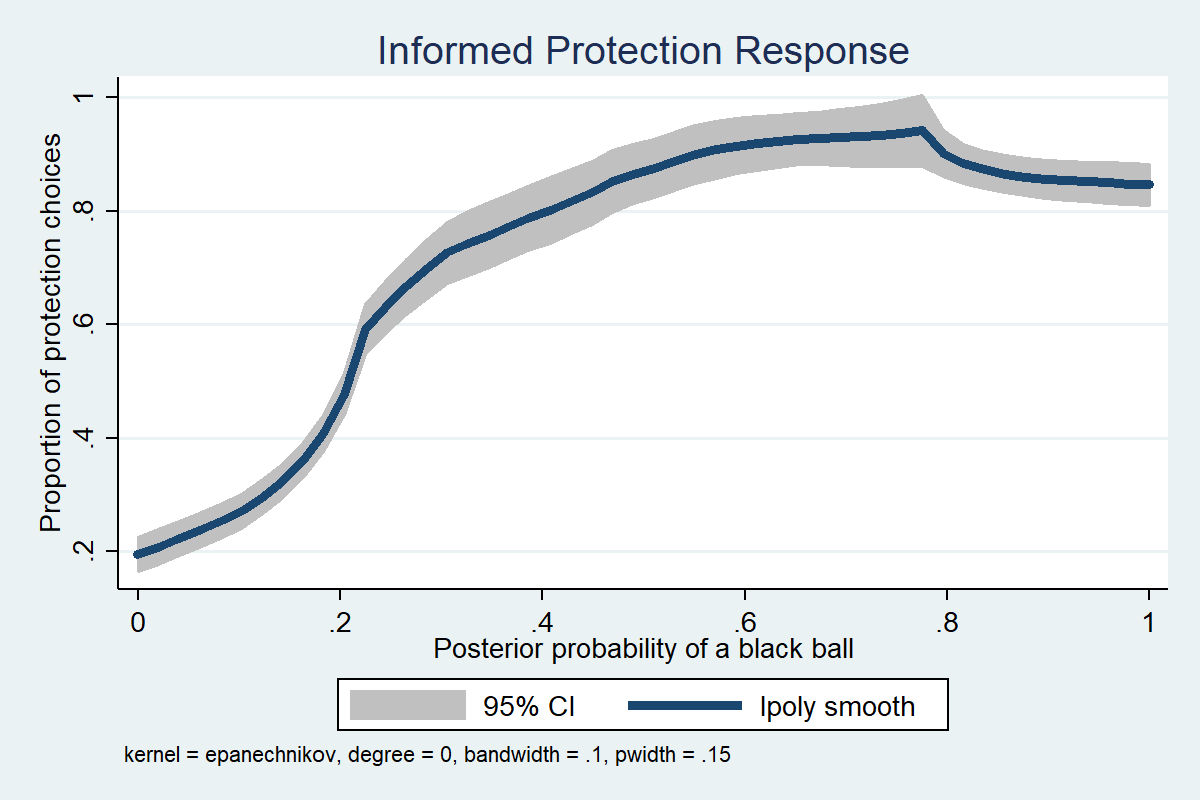
\includegraphics[width=\textwidth]{Graphs/ip_response_lpoly.png}
%
%\end{subfigure}
\end{figure}
\pmt{Eventually we need to add notes to the figures}
%%%%%%%%%%%%%%%%%%%%%%%%%%%%%%%%%%%%%%%%%%%%%%%%%%%%%%%%%%%%%%%%%%%%%%%%%%%%%%%%%%%%%%%%%%%%%%%%%%%%%%%%%%%%%%%%%%%

%\bigskip\noindent\textbf{Belief Elicitation.}\ \ \ 
\subsection{Belief Elicitation}
While the IP task gives us a sense for how subjects utilize signals in making protection decisions, we observe only whether or not they choose to protect, which conflates preferences with potential errors in updating posteriors.  The BP task gives provides insight into subjects' risk preferences, while the BE task allows us to better understand to what extent updating errors influence decisions.  

We define updating errors as the difference between the posterior and subjects’ elicited belief on the posterior probability of a black ball for a given signal.  We plot the distribution of the updating errors in the left hand column of Figure~\ref{fig:BeliefUpdate}, while the right hand column provides a scatter plot of the elicited beliefs against the true posterior with a fitted line.\pmt{I would prefer to take the r-squared out of this figure and put it in the table note with the correlations for each panel}\aut{Duly noted, will be incorporated.}.
%Since subjects were only given signal characteristics and not true posteriors, their IP responses reflect, inter alia, their ability to infer the true posteriors from signal characteristics. (I'm not sure I like my sentence better)
Panel A of Figure~\ref{fig:BeliefUpdate} uses all elicited beliefs and suggests that, while errors occur, beliefs are still sensible. The distribution of updating errors is centered at 0, with roughly one-half (51\%) concentrated within +/- 0.1 interval around zero. Overall, the correlation between the elicited beliefs and the true posteriors was 0.653.  

Using all the observations, however, obscures an important distinction: in many cases the ball color is completely certain based on priors and signals and so the updating should be trivial.  Panel B of Figure~\ref{fig:BeliefUpdate} includes only those 44\% beliefs elicited for an uncertain posterior. The median error is now -0.12, with with 90\% of errors between -0.48 and 0.3, suggesting that subjects tend to overestimate the likelihood of adverse events for uncertain posteriors, \pmt{which is consistent with what we see in Figure~\ref{fig:ProtResponse}}. The correlation between beliefs and posteriors in this subset of observations is only 0.571.  Panel C of Figure~\ref{fig:BeliefUpdate} plots the distribution of updating errors with certain posteriors, which includes: (i) treatments with all-honest gremlins; and (ii) treatments with obviously irrelevant dishonest gremlins (e.g., a group with honest and white-eyed gremlins with a hint that the ball is black — or vice versa). Reassuringly, 69\% of reported beliefs are correct, but subjects still err in about 30\% of cases. About half of these errors involve reporting a probability of between one and zero, with the other half reporting a probability of one when it should have been zero. \aut{There is little evidence of these drastic errors (0 instead of 1) being strongly correlated with randomness in other treatments.} \pmt{It depends a bit.  Are some guys doing everything right here and others doing everything wrong?  Is there any relationship between errors here and inconsistencies in BP or a lower correlation between BP and IP tasks?} 

\pmt{I'm leaving this here because I'm not really sure what to do with it.  I like being able to say that our results are consistent with previous literature, but I don't know this literature, especially Mobius (2011).}\aut{Not sure we should go in this direction:}Overall, the pattern of belief updating is consistent with previous literature which finds that while humans update beliefs in a correct direction, they tend to underaccount both the effect of prior probabilities and the effect of signals (--my citations--). The first effect received the name of base-rate neglect, while the latter is called signal underweighting. These effects lower the correlation between posteriors and reported beliefs and reduce sensitivity of beliefs to signal characteristics. Using the standard approach of Mobius (2011), we find that --- 

\aut{Here is my fist take on the presentation order problem - higher priors.}
\textbf{We also observe that subject underestimate posterior probabilities more when facing prior probabilities of 0.3 and 0.5 with the differences being statistically significant} at significance level 0.05 \aut{I guess, I should add a table here}\pmt{Can you do a figure that breaks out the error distributions for the lower priors and the higher priors?}. We cannot however exclude that it happens due to presentation order effects: subjects face priors 0.3 and 0.5 in the second part of experiment with some subjects failing to account for higher priors. Indeed, nine subjects do not change their responses between priors at all (so all six responses for higher priors are the same), but only two do not change their responses with signals\pmt{Related to my comment above, can we identify guys who are total knuckleheads across all tasks using this failure to change with priors?  For instance, are all of these 9 guys multiple switchers in BP and making errors when the posterior is certain in BE?}. \pmt{I would delete this next sentence, or at least move most of it, because we haven't talked about WTP yet.}We observe similar pattern in the Willingness-to-Pay Elicitation task with thirteen subjects not updating their willingness-to-pay. For this reason, we have decided to exclude higher priors from the rest of the analysis limiting our sample only to one prior per subject (0.1 or 0.2).
\pmt{I think this is the appropriate place to address the order effect, but I haven't addressed it further because of the questions I asked above}
%%%%%%%%%%%%%%%%%%%%%%%%%%%%%%%%%%%%%%%%%%%%%%%%%%%%%%%%%%%%%%%%%%%%%%%%%%%%%%%%%%%%%%%%%%%%%%%%%%%%%%%%%%%%%%%%%%%

\begin{figure}[H]
	\centering
	\caption{Errors in Bayesian Updating} \label{fig:BeliefUpdate}
	\subcaptionbox{Error Distribution}{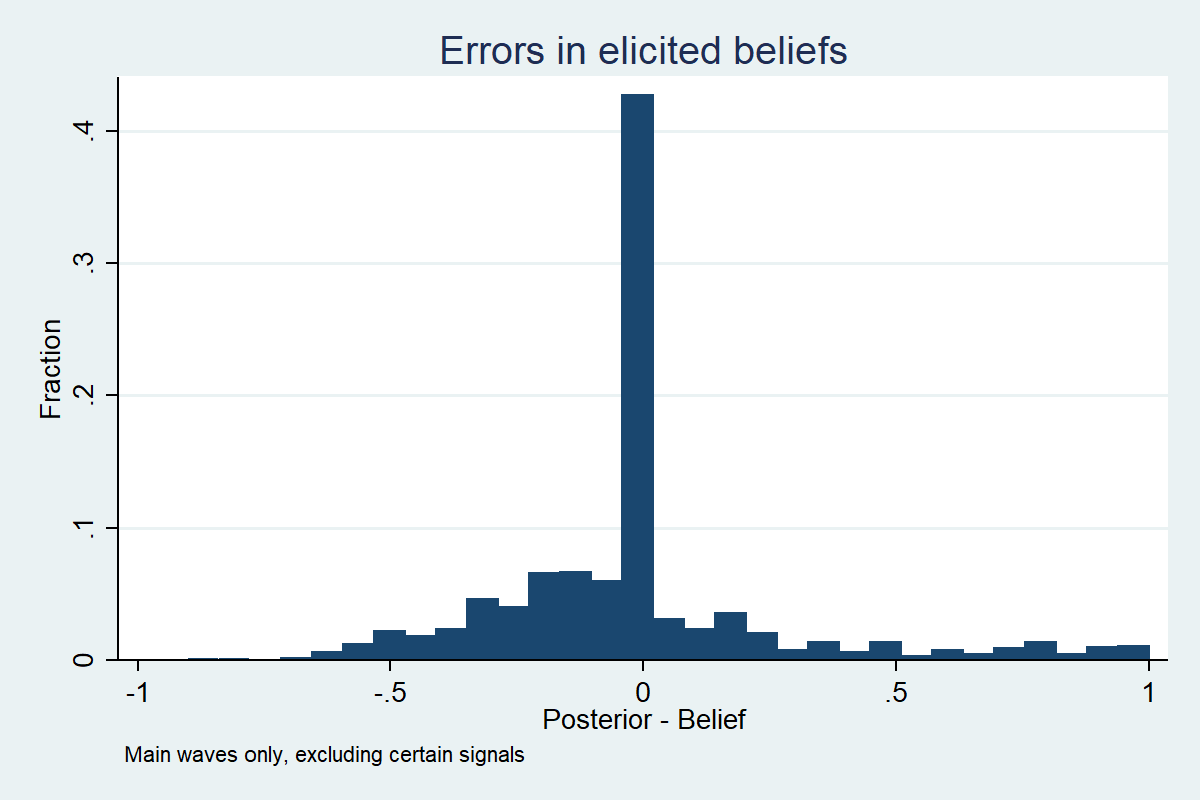
\includegraphics[width=.48\textwidth]{Graphs/hist_belief_error_s3.png}}
	\hfill
	\subcaptionbox{Error v. Posterior}{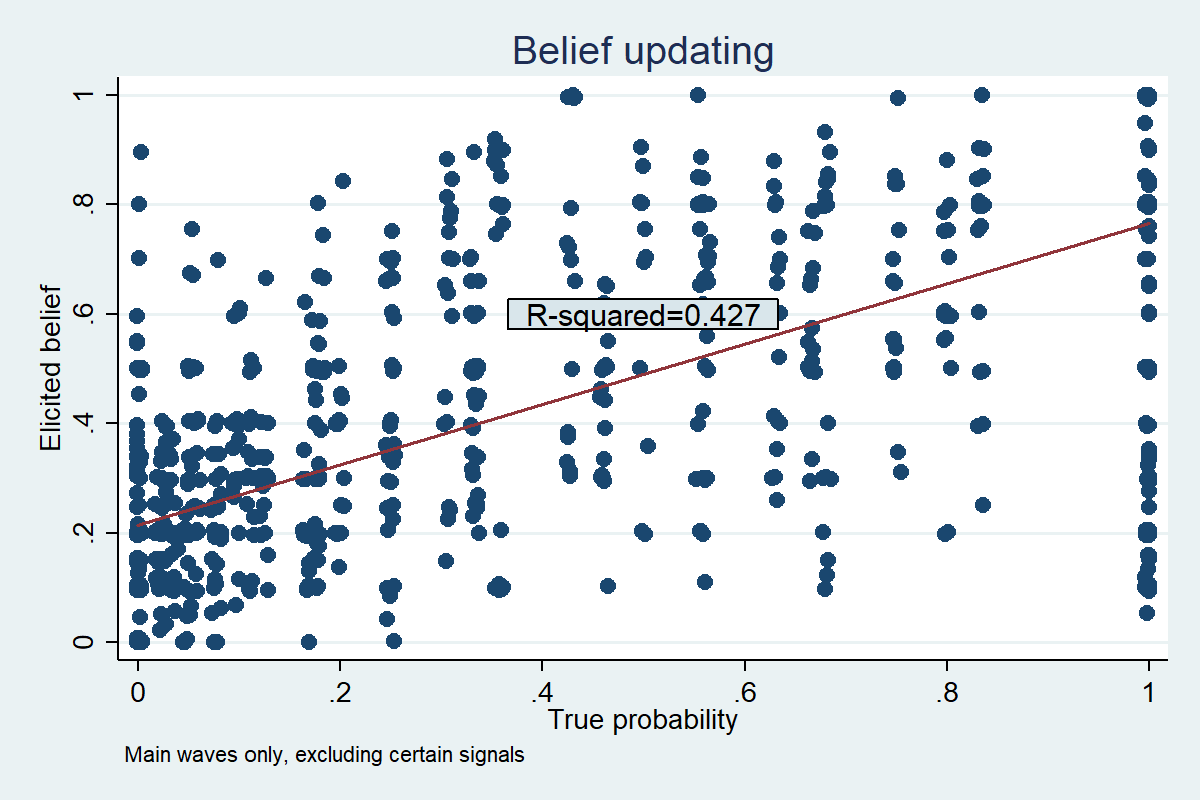
\includegraphics[width=.48\textwidth]{Graphs/updating_s3.png}}
	\hfill
	\subcaptionbox{Error Distribution, Uncertain Color}{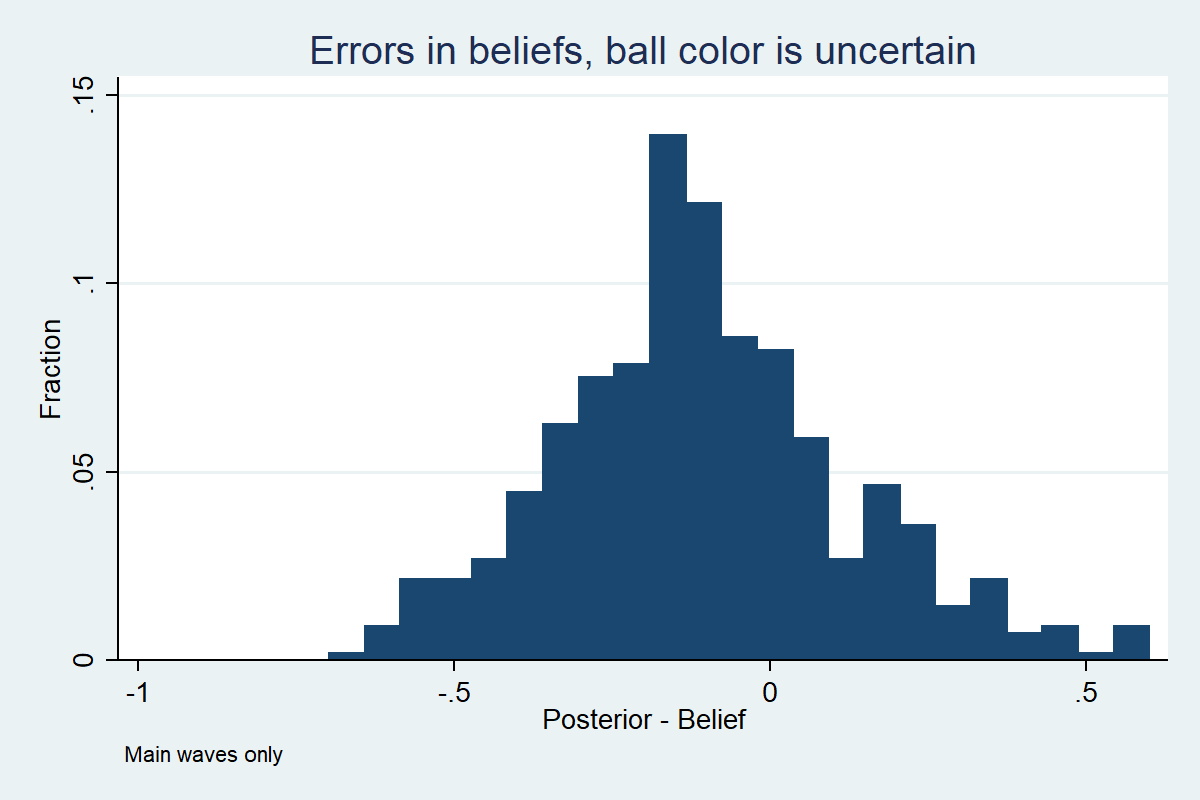
\includegraphics[width=.48\textwidth]{Graphs/hist_belief_error_s4.png}}
	\hfill
	\subcaptionbox{Error v. Posterior, Uncertain Color}{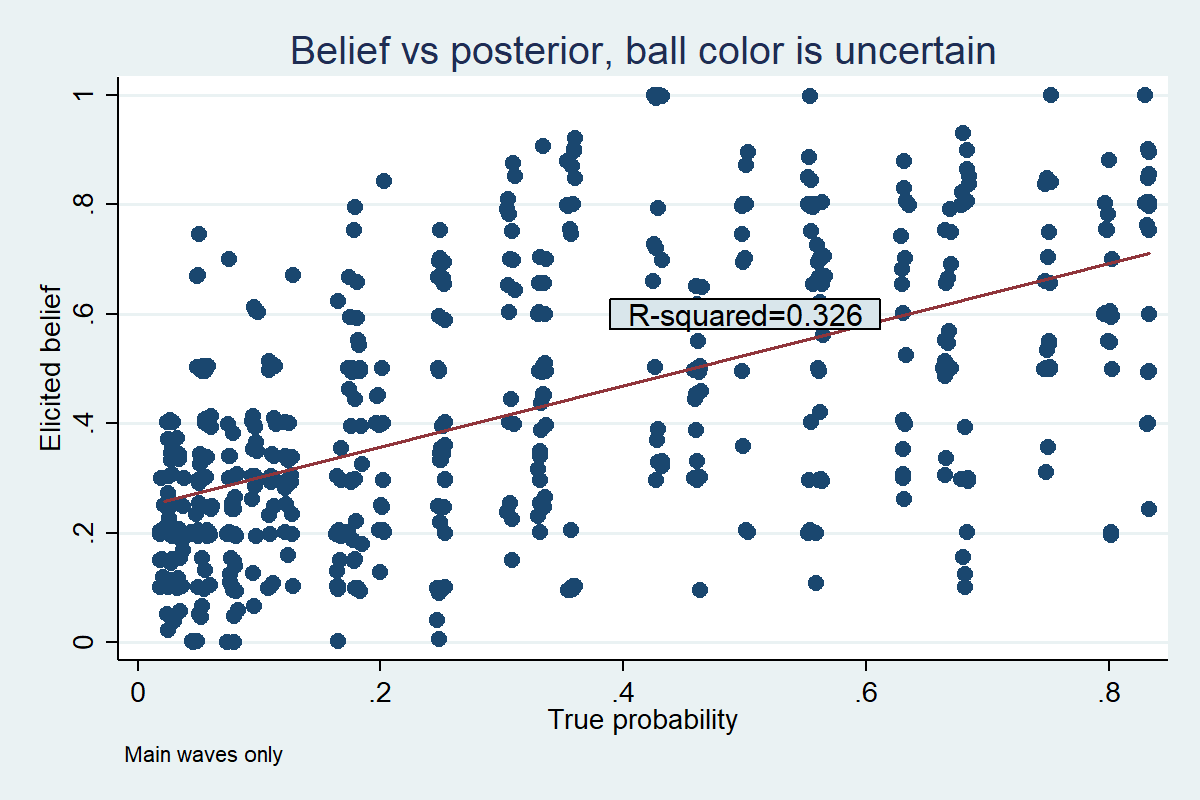
\includegraphics[width=.48\textwidth]{Graphs/updating_s4.png}}
	\hfill
	\subcaptionbox{Error Distribution, Certain Color}{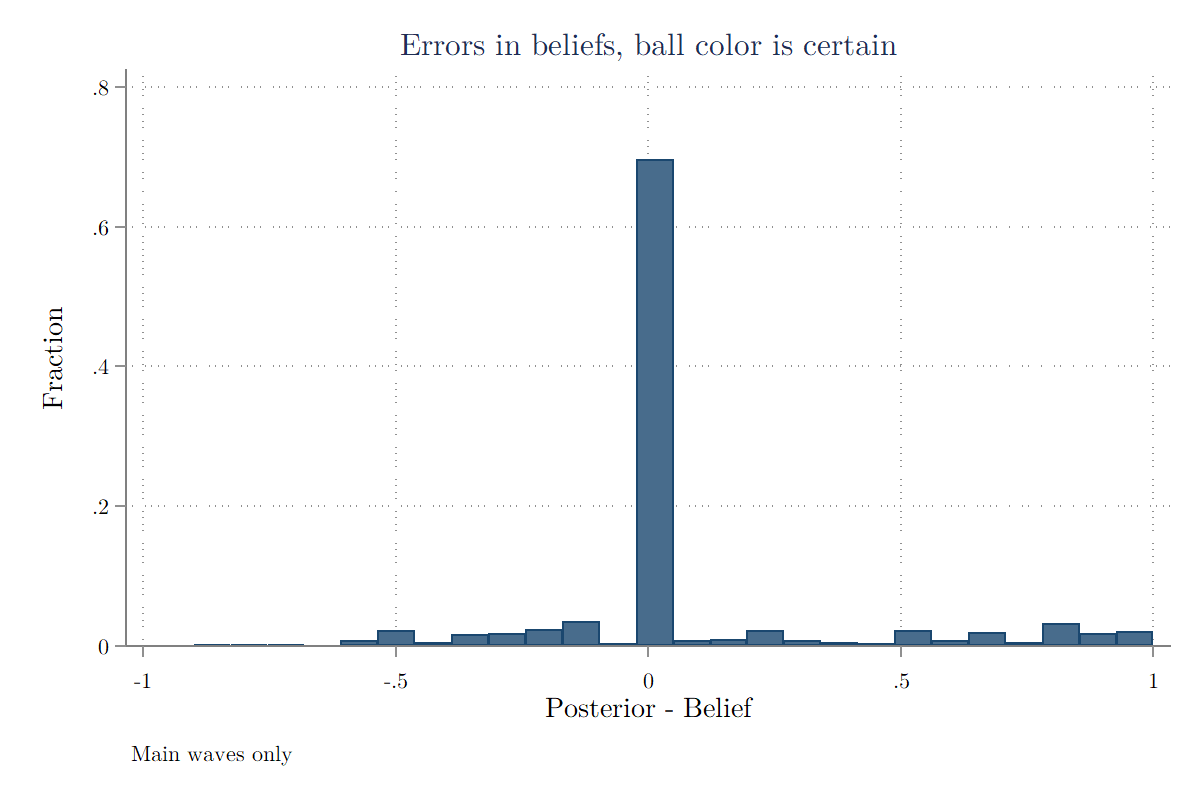
\includegraphics[width=.48\textwidth]{Graphs/hist_belief_error_s5.png}}
	\hfill
	\subcaptionbox{Error v. Posterior, Certain Color}{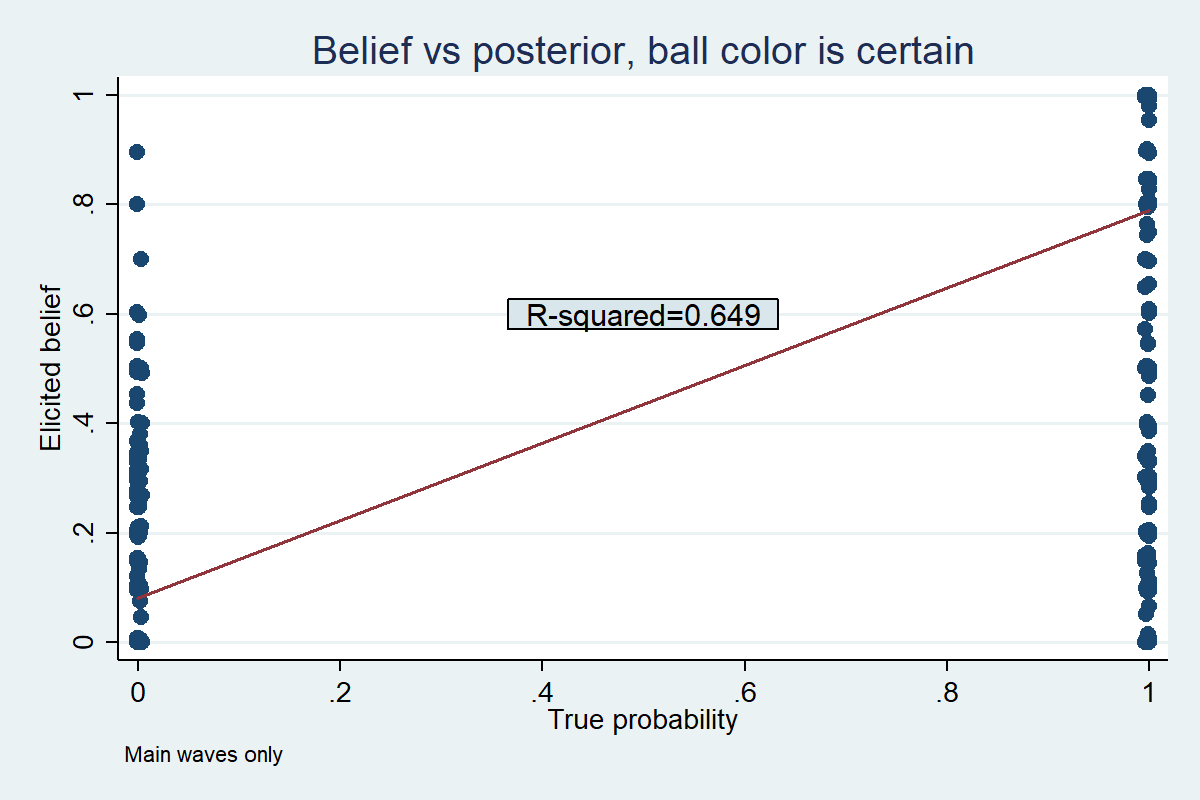
\includegraphics[width=.48\textwidth]{Graphs/updating_s5.png}}
	\hfill
\end{figure}
\clearpage

%%%%%%%%%%%%%%%%%%%%%%%%%%%%%%%%%%%%%%%%%%%%%%%%%%%%%%%%%%%%%%%%%%%%%%%%%%%%%%%%%%%%%%%%%%%%%%%%%%%%%%%%%%%%%%%%%%%

%\bigskip\noindent\textbf{Willingness-to-Pay Elicitation.}\ \ \ 
\subsection{Willingness-to-Pay Elicitation}
The BP, IP, and BE tasks allow us to discern how individuals use freely provided information to make protection decisions, but signals are not necessarily provided freely.  To be better understand how subjects value the signals, we elicit their Willingness-to-Pay for signals of differing degrees of informativeness.  Figure XX plots the distributions of the theoretically optimal WTP\pmt{We should explain here where this comes from} (Panel A), the distribution of actually WTP (Panel B), and the distribution of the discrepancies between the theoretical and actual WTP that we observe.  WTP to pay is bounded between \$0 and \$5, where the latter is because protection can be purchased for \$5 so if information were that valuable, an individual would just choose to protect.  \pmt{Placeholder for where we say something about my suggested Panels A and B.}  The theoretical WTP is a useful benchmark, as XX\% of the actual WTP are within \$0.50 of the theoretical WTP.  Nonetheless, there is substantial variation in the discrepancies between actual and theoretical WTP, and there are both substantial fractions of subjects who overpay (XX\% overpay by \$1 or more) and underpay (XX\% underpay by \$1 or more).


%\subsection{Signal Characteristics and Protection Decision}
\section{Signal characteristics and protection decisions} 
\pmt{I like this structure, but eventually I think we want to put the hypotheses in an earlier section (e.g., with the model)}
\begin{hypothesis} Conditional on posterior probability of a black ball, signal characteristics do not affect protection decisions. \end{hypothesis}
\begin{result}\label{res:IPdeviations} %Signal characteristics affect protection decision.
Conditional on posterior probability of a black ball, subjects' protection decisions still respond to the signals' false positive and false negative rates. \end{result}

in Table~\ref{tab:nonparIP} we break out average protection decisions by signal characteristics.\pmt{Do we need the ``Row" column?  It certainly makes referencing the table easier, but it also makes the table one column wider.} The first three columns summarize the information available to the subject, i.e., the signal as well as whether the signal might be either a false positive or false negative. Column 4 shows the posterior probability of a black ball averaged across all the treatments within a group, Column 5 the share protection among actual IP responses, Column 6 the p-value of a \emph{t-}test that the protection probability is zero.\aut{On a second thought, it doesn't make sense. It cannot be zero if someone protected.}, Column 7 the share of protection under the RN optimum, and Column 8 the p-value of a \emph{t-}test that actual and optimal choices use the same probability of protection.

First, we note that regardless of FP and FN rates, a hint that the ball is black substantially increases the share of protection decisions.  \textbf{Second, subjects' protection decisions in the majority of treatments significantly deviate from what is optimal for risk-neutral subjects.}  In general, subjects tend to overprotect when facing white signals (rows 1--4) and underprotect when facing black signals (rows 5--8). The exceptions are treatments with black signals and positive FP rates in which we cannot reject the hypothesis that the protection responses matches the response of a risk-neutral subject. 

\textbf{In light of BP decisions it is not surprising that subjects do not behave as risk-neutral agents, but several of deviations from the RN optimal behavior cannot be explained by the expected utility maximization for any degree of risk aversion.} For example, consider the change in the protection rates between rows 1 and 3: the signal is white, so an increase in the signal's FP rate does not change the posterior, but the protection rate increases by more than 11 percentage points (pp.). Similarly, row 4 shows that when both FP and FN are positive, the protection rate increases to 43 percent --- even though the average (maximum) posterior probability for the signal characteristics is 6\pmt{What is this? ~(11)} percent. As a benchmark, with no signal in the BP task, only 13~(32) percent of subjects chose to protect when the probability is 10~(15) percent. 

%%%%%%%%%%%%%%%%%%%%%%%%%%%%%%%%%%%%%%%%%%%%%%%%%%%%%%%%%%%%%%%%%%%%%%%%%%%%%%%%%%%%%%%%%%%%%

\begin{table}[H]\centering 
\caption{Average Protection by Signal Type} 
\label{tab:nonparIP}
\adjustbox{max width=\textwidth}{
	\begin{threeparttable}
	\begin{tabular}{ccccccccc} \hline \hline
	\multirow{4}{6ex}{\centering \textbf{Row}}
			&\multicolumn{3}{c}{\centering \textbf{Signal Characteristics}} 
			& \multirow{3}{10ex}{\centering \textbf{Posterior}} & \multirow{3}{10ex}{\centering \textbf{Share Protect}} 
			& \multirow{3}{13ex}{\centering \textbf{P-val $(H_0: ShProt = 0)$}} 
			& \multirow{3}{10ex}{\centering \textbf{Share Optimal}} 
			& \multirow{3}{13ex}{\centering \textbf{P-val $(H_0: ShProt=ShOptimal)$}} \\ 
			\cmidrule(lr){2-4}
		&\multirow{2}{10ex}{\centering \textbf{False Positive}} & \multirow{2}{12ex}{\centering \textbf{False Negative}} 
			& \multirow{2}{10ex}{\centering \textbf{Signal}} 
		\\
		\\
		&(1) & (2) & (3) & (4) & (5) & (6) & (7) & (8) \\
		\hline
			(1)&No&No  &White&0.000&0.067&0.000&0.000\\
(2)&No&Yes &White&0.100&0.333&0.000&0.000\\
(3)&Yes&No &White&0.000&0.130&0.000&0.000\\
(4)&Yes&Yes&White&0.131&0.564&0.121&0.000\\
(5)&No&No  &Black&1.000&0.846&1.000&0.000\\
(6)&No&Yes &Black&1.000&0.841&1.000&0.000\\
(7)&Yes&No &Black&0.550&0.833&0.870&0.355\\
(8)&Yes&Yes&Black&0.483&0.886&0.871&0.685\\

			\\
		\hline\hline 
	\end{tabular} 
	\begin{tablenotes}[flushleft]
			\item\leavevmode\kern-\scriptspace\kern-\labelsep \footnotesize \textit{Notes:} 
	\end{tablenotes}								
	\end{threeparttable}
	}
\end{table}



%%%%%%%%%%%%%%%%%%%%%%%%%%%%%%%%%%%%%%%%%%%%%%%%%%%%%%%%%%%%%%%%%%%%%%%%%%%%%%%%%%%%%%%%%%%%%


\begin{hypothesis} Subjects' Bayesian-updating errors explain IP decisions. \end{hypothesis}
\pmt{Should this be something like ``updating errors explain IP decisions, and updating errors are influenced by signal characteristics?}
\begin{result} When subjects received a signal that the ball is white, the signal's false positive and false negative rates biased their belief upward. When subjects received a signal that the ball is black, the signal's false positive (negative) rates biased their belief upward (downward). Updating errors provide partial explain for subjects' IP decisions conditional on posterior.\end{result}

\textbf{We observe that many IP responses cannot be reconciled with expected utility maximization given posterior probability, but EU maximization could break down if subjects fail to correctly estimate posteriors.} Table~\ref{tab:nonparError} summarizes how the updating errors vary with signal characteristics. We find that subjects overestimate the probability of a black ball with a white signal. Introducing FP rates to the signal exacerbated their upward bias. To illustrate, consider the change between rows 1 and 3, where introducing a FP rate would not change the posterior because the signal is white. Yet, subjects update their posterior upward, magnifying their updating error. The FN rates also have a similar effect of exacerbating this upward bias for a white signal.

The updating bias for black signals, however, varies by information structure. When there is no risk of a false-positive signal (rows 5-6), subjects underestimate the probability of a black ball after receiving a black signal. \aut{Not sure we need it here: This observation contrasts with the case of the white signal, for which introducing FP rates led subjects to overestimate the posterior instead.} Subjects slightly underestimate the probability even when the signal is honest, but introducing FN rates lead subjects to underestimate it further. To illustrate, the introduction of a FN rate given a black signal does not change the posterior rows 5 and 6, but subjects decrease their beliefs. When there is a risk of a false-positive (i.e., FP$>$0), subjects again overestimate the probability of a black ball with little difference in errors between treatments with FP events only and with both FP and FN events. It seems that, because the false-positive rate negatively affects the posterior, subjects fail to adjust their beliefs enough in response to FP rates.

Table~\ref{tab:updateErrorReg} formalizes our analysis using a regression which allows to implicitly contol for risk aversion\pmt{this also controls for a general inability to update though, right?} through subject fixed effects. We estimate a linear regression of updating error (actual posterior - reported belief) on FP and FN rates by signal color. It provides support for the conclusions from Table~\ref{tab:nonparError}: (i) subjects make positive (negative) updating errors for white (black) signals; (ii) FP rates induce an upward bias in subjects' estimates of the posterior; and (iii) FN rates induce an upward (downward) bias when the signal is white (black). This pattern can explain overprotection in the IP task with white signals when the FP rate is positive.


%%%%%%%%%%%%%%%%%%%%%%%%%%%%%%%%%%%%%%%%%%%%%%%%%%%%%%%%%%%%%%%%%%%%%%%%%%%%%%%%%%%%%%%%%%%%%

\begin{table}[H]\centering 
\caption{Average Updating Error by Signal Type} 
\label{tab:nonparError}
\adjustbox{max width=\textwidth}{
	\begin{threeparttable}
	\begin{tabular}{ccccccc} 
	\hline \hline
 \multirow{4}{6ex}{\centering \textbf{Row}}& \multicolumn{3}{c}{\centering \textbf{Signal Characteristics}}
			& \multirow{3}{10ex}{\centering \textbf{Posterior}}  
			& \multirow{3}{12ex}{\centering \textbf{Updating Error$^*$}} & \multirow{3}{12ex}{\centering \textbf{P-val $(H_0: Error = 0)$}}  \\ \cmidrule(lr){2-4}
		& \multirow{2}{10ex}{\centering \textbf{False Positive}} & \multirow{2}{12ex}{\centering \textbf{False Negative}} 
			& \multirow{2}{10ex}{\centering \textbf{Signal}} 
		\\
		\\
		& (1) & (2) & (3) & (4) & (5) \\
	
		\hline	
1&No&No&White&0.000&0.039&0.001\\
2&No&Yes&White&0.045&0.140&0.000\\
3&Yes&No&White&0.000&0.116&0.000\\
4&Yes&Yes&White&0.062&0.245&0.000\\
5&No&No&Black&1.000&-0.187&0.000\\
6&No&Yes&Black&1.000&-0.332&0.000\\
7&Yes&No&Black&0.396&0.177&0.000\\
8&Yes&Yes&Black&0.328&0.192&0.000\\
\\ 	[-1em]
\hline\hline
\end{tabular} 
	\begin{tablenotes}[flushleft]
			\item\leavevmode\kern-\scriptspace\kern-\labelsep \footnotesize \textit{Notes:} $^* \text{Updating error} = Posterior - Belief$. 
	\end{tablenotes}								
	\end{threeparttable}
	}
\end{table}
%%%%%%%%%%%%%%%%%%%%%%%%%%%%%%%%%%%%%%%%%%%%%%%%%%%%%%%%%%%%%%%%%%%%%%%%%%%%%%%%%%%%%%%%%%%%%


%%%%%%%%%%%%%%%%%%%%%%%%%%%%%%%%%%%%%%%%%%%%%%%%%%%%%%%%%%%%%%%%%%%%%%%%%%%%%%%%%%%%%%%%%%%%%

\begin{table}[htbp]\centering 
\caption{Updating Errors in BE Task} 
\label{tab:updateErrorReg}
\adjustbox{max width=\textwidth}{
	\begin{threeparttable}
	\begin{tabular}{l*{3}{c}}
	\hline\hline
									&\multirow{2}{8ex}{\centering All}&\multicolumn{2}{c}{Signal Received}\\ \cmidrule{3-4}
									&&\multicolumn{1}{c}{White}&\multicolumn{1}{c}{Black}\\
									&\multicolumn{1}{c}{(1)}&\multicolumn{1}{c}{(2)}&\multicolumn{1}{c}{(3)}\\
	\hline

	FP rate         &     .948\sym{***}&     .318\sym{***}&     1.58\sym{***}\\
                &    (0.1)         &    (0.1)         &    (0.1)         \\
FN rate         &   .00702         &      .38\sym{***}&    -.366\sym{***}\\
                &    (0.1)         &    (0.1)         &    (0.1)         \\
Constant        &    -.249\sym{***}&     .139\sym{***}&    -.636\sym{***}\\
                &    (0.0)         &    (0.0)         &    (0.0)         \\
\hline
Observations    &      624         &      312         &      312         \\
Adjusted \(R^{2}\)&     0.22         &     0.37         &     0.66         \\

	\\ [-1em]
	\hline
	Subject FE      &      Yes         &      Yes         &      Yes         \\
	\hline
	\hline\hline
	\end{tabular}
	\begin{tablenotes}[flushleft]
			\item\leavevmode\kern-\scriptspace\kern-\labelsep \footnotesize \textit{Notes:} Standard errors in parentheses. \sym{*} \(p<0.10\), \sym{**} \(p<0.05\), \sym{***} \(p<0.01\). 
	\end{tablenotes}								
	\end{threeparttable}
	}
\end{table}


%%%%%%%%%%%%%%%%%%%%%%%%%%%%%%%%%%%%%%%%%%%%%%%%%%%%%%%%%%%%%%%%%%%%%%%%%%%%%%%%%%%%%%%%%%%%%



\textbf{So far, errors in the posterior estimation seem to be consistent with biases observed in the Informed Protection task. It begs the questions of how much bias in the IP task remains after accounting for biases in beliefs.} In Table~\ref{tab:protectReg}, we regress informed protection decisions on FP and FN rates and flexible controls of both posteriors and reported beliefs:

	\[Prob(s_{ij}=1)=Logit(\alpha_i+\beta_1 FP +\beta_2 FN +Z(p_{ij})+Z(\mu_{ij})+\epsilon_{ij}) \]
where $s_{ij}$ is the protection decision of subject $i$ in treatment $j$, $\alpha_i$ - subject FE, $P_{10}$, $P_{01}$ are FP and FN false positive and false negative rates and $Z(p_{ij}),Z(\mu_{ij})$ are vectors of flexible controls\pmt{We probably need a more plain language explanation than just the footnote}\footnote{We use Stata mkspline command to create flexible controls as 5 splines $z_1(x),z_2(x),..z_5(x)$ of initial variable $x$ over the range $[0,1]$ such that $z_k(x)=\min[0,x-x_{k-1},x_k-x_{k-1}]$ with $x_k$ being equally spaced knot values. Splines account for potential nonlinear effects of posteriors and beliefs on protection decision with limited effect on degrees of freedom.} of posteriors and reported beliefs $\mu_{ij}$ for corresponding treatments. Columns 1 and 2 include only the flexible controls of the true posteriors. Columns 3 and 4 add further flexible controls to account for subjects' (often incorrect) estimates of the posterior, inferred from their BE responses. The model is estimated using Maximum Likelihood Estimation, with standard errors clustered at the subject level. The table presents the average marginal effect coefficients.

Columns 1 and 2 confirmed Result~\ref{res:IPdeviations}, to wit, conditional on posterior and subject FE, IP responses are affected by FP and FN rates. For a white signal, FP and FN rates increased the tendency to overprotect; while for a black signal, FP rate had an opposite effect with comparable magnitude but without statistical significance. Column 3 suggests, however, that once we control for both the posterior and subjects' updated belief, only the effect of the FP rate for white signals remains positive and statistically significant at $p<0.1$. \textbf{These results provide evidence that subjects' failure to protect optimally is largely --- albeit not entirely --- driven by their failure to correctly update their posterior given a signal.}

\agt{XXX DO WE NEED COLUMNS 2 and 4? XXX NOT SURE...}


%%%%%%%%%%%%%%%%%%%%%%%%%%%%%%%%%%%%%%%%%%%%%%%%%%%%%%%%%%%%%%%%%%%%%%%%%%%%%%%%%%%%%%%%%%%%%
\begin{table}[htbp]\centering 
\caption{Informed Protection Response} 
\label{tab:protectReg}
\adjustbox{max width=\textwidth}{
	\begin{threeparttable}	
	\begin{tabular}{l*{4}{c}}
	\hline\hline
									&\multicolumn{1}{c}{(1)}&\multicolumn{1}{c}{(2)}&\multicolumn{1}{c}{(3)}&\multicolumn{1}{c}{(4)}\\
	\hline
		
		FP rate x (S=White)&     .676\sym{***}&     .552\sym{**} &     .379\sym{*}  &     .309         \\
                &    (3.5)         &    (2.2)         &    (1.9)         &    (1.2)         \\
FN rate x (S=White)&     1.08\sym{**} &     1.57\sym{***}&     .583         &     1.04\sym{**} \\
                &    (2.3)         &    (3.3)         &    (1.2)         &    (2.1)         \\
S=Black         &      1.2\sym{**} &     2.13\sym{***}&     .706         &     1.56\sym{***}\\
                &    (2.1)         &    (3.8)         &    (1.3)         &    (2.7)         \\
FP rate x (S=Black)&    -.887         &    -1.57\sym{*}  &    -.507         &    -1.05         \\
                &   (-1.0)         &   (-1.9)         &   (-0.6)         &   (-1.4)         \\
FN rate x (S=Black)&   -.0383         &    -.372\sym{*}  &   -.0542         &    -.372\sym{*}  \\
                &   (-0.3)         &   (-1.9)         &   (-0.3)         &   (-1.7)         \\
p$=$0.2         &     .404\sym{***}&     .363\sym{***}&     .357\sym{***}&     .316\sym{***}\\
                &    (9.5)         &    (7.1)         &    (7.1)         &    (5.0)         \\
FP rate x (p=0.2)&                  &      .55\sym{*}  &                  &     .405         \\
                &                  &    (1.7)         &                  &    (1.2)         \\
FN rate x (p=0.2)&                  &     .518\sym{*}  &                  &      .52\sym{*}  \\
                &                  &    (1.8)         &                  &    (1.8)         \\
\hline
N               &      582         &      582         &      582         &      582         \\
Pseudo R-squared&     .575         &     .585         &     .609         &     .617         \\
Log-likelihood  &     -172         &     -168         &     -158         &     -154         \\
	
	\\ [-1em]
	\hline
	Subject FE & Yes & Yes & Yes & Yes \\
	Flexible controls for: \\
	\hspace{1.5ex} Posterior & Yes & Yes & Yes & Yes \\
	\hspace{1.5ex} Beliefs & No & No & Yes & Yes \\	
	\hline\hline
	\end{tabular}
	\begin{tablenotes}[flushleft]
			\item\leavevmode\kern-\scriptspace\kern-\labelsep \footnotesize \textit{Notes:} Coefficients are average marginal effects. \emph{t}-statistics in parentheses. Standard errors are clustered at the subject level. \sym{*} \(p<0.10\), \sym{**} \(p<0.05\), \sym{***} \(p<0.01\). 
	\end{tablenotes}								
	\end{threeparttable}
	}
\end{table}



%%%%%%%%%%%%%%%%%%%%%%%%%%%%%%%%%%%%%%%%%%%%%%%%%%%%%%%%%%%%%%%%%%%%%%%%%%%%%%%%%%%%%%%%%%%%%


\newpage\clearpage

\agt{XXX ARYA STOPPED HERE XXX}

%\subsection{Willingness to Pay}

%Figure XX shows how subjects deviate substantially from the theoretical value for a risk-neutral subject. Here we explore these deviations more systematically by signal characteristics and risk preferences. 

We have shown that signal characteristics both indirectly (through beliefs) and directly (white signals and false positives) influence protection decisions when signals are exogenously provided.  It is far from clear how signal characteristics should affect WTP decisions, however, where the theoretical benchmark had more limited explanatory power, and where any self-awareness of one's inability to update might limit the value of information.

Table XX provides some preliminary evidences that, not only do signal characteristics influence WTP, they do so systematically in a way that suggests subjects are not aware of their own biases.  When there is no possibility of a false positive, subjects underestimate the value of signal relative to the theoretical benchmark.  Regardless of the possibility of a false negative, this difference is not statistically significant at conventional significance levels, though it is both 55\% larger in magnitude and closer to significant ($p=0.152$) when there are false negatives.  When there are false positives, however, subjects significantly overvalue signals relative to the theoretical benchmark, and there is virtually no difference in magnitude between the cases where there are and are not false negatives.\pmt{Can we plot the distributions of deviations for these 4 cases?}

\pmt{WE NEED A GOOD SEGUE TO REGRESSION AND DISCUSSION OF RESULTS, BUT I HAVE STOPPED HERE IN THIS SECTION}

%%%%%%%%%%%%%%%%%%%%%%%%%%%%%%%%%%%%%%%%%%%%%%%%%%%%%%%%%%%%%%%%%%%%%%%%%%%%%%%%%%%%%%%%%%%%%%%%%

\begin{table}[htbp]\centering
\def\sym#1{\ifmmode^{#1}\else\(^{#1}\)\fi}
\caption{WTP for Information (tobit)}
\begin{tabular}{l*{6}{c}}
\hline\hline
                &\multicolumn{1}{c}{(1)}&\multicolumn{1}{c}{(2)}&\multicolumn{1}{c}{(3)}&\multicolumn{1}{c}{(4)}&\multicolumn{1}{c}{(5)}&\multicolumn{1}{c}{(6)}\\
                &\multicolumn{1}{c}{All}&\multicolumn{1}{c}{p=0.1}&\multicolumn{1}{c}{p=0.2}&\multicolumn{1}{c}{All}&\multicolumn{1}{c}{All}&\multicolumn{1}{c}{All}\\
\hline
model           &                  &                  &                  &                  &                  &                  \\
FN costs        &    -.577\sym{**} &    -1.24\sym{**} &    -.682\sym{***}&    -.791\sym{***}&    -.691\sym{***}&     -.69\sym{***}\\
                &    (0.2)         &    (0.5)         &    (0.3)         &    (0.2)         &    (0.2)         &    (0.3)         \\
FP costs        &    -.644\sym{***}&    -.647\sym{***}&    -.519\sym{**} &    -.595\sym{***}&    -.508\sym{***}&    -.494\sym{**} \\
                &    (0.2)         &    (0.2)         &    (0.3)         &    (0.2)         &    (0.2)         &    (0.2)         \\
BP costs        &                  &                  &                  &     .373\sym{***}&     .363\sym{***}&      .37\sym{***}\\
                &                  &                  &                  &    (0.1)         &    (0.1)         &    (0.1)         \\
Belief change   &                  &                  &                  &                  &     .332         &                  \\
                &                  &                  &                  &                  &    (0.3)         &                  \\
Certainty       &                  &                  &                  &                  &                  &     .688         \\
                &                  &                  &                  &                  &                  &    (0.8)         \\
Constant        &     1.98\sym{***}&     1.79\sym{***}&     2.33\sym{***}&     .923\sym{***}&     .701\sym{*}  &     .293         \\
                &    (0.2)         &    (0.2)         &    (0.2)         &    (0.3)         &    (0.4)         &    (0.8)         \\
\hline
sigma           &                  &                  &                  &                  &                  &                  \\
Constant        &      1.8\sym{***}&     1.83\sym{***}&      1.7\sym{***}&     1.77\sym{***}&     1.76\sym{***}&     1.76\sym{***}\\
                &    (0.1)         &    (0.1)         &    (0.1)         &    (0.1)         &    (0.1)         &    (0.1)         \\
\hline
Observations    &      312         &      159         &      153         &      312         &      312         &      312         \\
Adjusted \(R^{2}\)&                  &                  &                  &                  &                  &                  \\
\hline\hline
\multicolumn{7}{l}{\footnotesize Standard errors in parentheses}\\
\multicolumn{7}{l}{\footnotesize \sym{*} \(p<0.10\), \sym{**} \(p<0.05\), \sym{***} \(p<0.01\)}\\
\end{tabular}
\end{table}



In Table XX, we use a regression analysis to investigate how and why subjects deviate from the risk-neutral subjects’ theoretical WTP for a signal of a given quality (conditional on prior). We first estimate how individual deviations from the theoretical benchmark $b^*_s$ for a given signal $s$ are correlated with signal's charactaristics:

\[b_{is} - b^*_s = \beta_0 + \beta_1 FalsePositive + \beta_2 FalseNegative + \epsilon_{is}\]
where $b_{is}$ is the reported WTP of individual $i$ for treatment $s$ and $b^*_s$ is the signal's value for a risk-neutral subject, and FalsePositive (FalseNegative) is the false positive (false positive) costs variables that captures signal quality. We calculate false positive costs as the product of prior probability of a white ball multiplied by the conditional probability of getting a black signal (“The ball is black!”) from a randomly chosen gremlin: $FalsePositive=(1-\pi) P_{10}c$. Similarly we calculate false negative costs as the probability of an adverse state multiplied by a conditional probability of getting a white signal conditional on the ball being black and multiplied by potential loss $FalseNegative=\pi P_{01}L$. Note that these costs already account for expected frequency of receiving different incorrect signals as consistent with their base rate. If our subjects were risk neutral expected utility maximizers, we expect $\beta_1$ and $\beta_2$ to be zero.

%%%%%%%%%%%%%%%%%%%%%%%%%%%%%%%%%%%%%%%%%%%%%%%%%%%%%%%%%%%%%%%%%%%%%%%%%%%%%%%%%%%%%%%%%%%%%%%%%
\begin{table}[H]\centering \caption{Average WTP discrepancy (WTP-Value) by Signal Type} 
\label{tab:WTP_nonpar}
\begin{tabular}{cccc} \hline \hline
\textbf{False-positive}&\textbf{False-negative}&\textbf{Mean WTP discrepancy}& \textbf{P($=0$)}\\ \hline
No&No&-0.106&0.433\\
No&Yes&0.143&0.250\\
Yes&No&0.081&0.502\\
Yes&Yes&0.492&0.000\\
\hline \end{tabular} \end{table}

\begin{table}[H]\centering
\def\sym#1{\ifmmode^{#1}\else\(^{#1}\)\fi}
\caption{WTP minus Value of Information (OLS)}
\begin{tabular}{l*{5}{c}}
\hline\hline
                &\multicolumn{1}{c}{(1)}&\multicolumn{1}{c}{(2)}&\multicolumn{1}{c}{(3)}&\multicolumn{1}{c}{(4)}&\multicolumn{1}{c}{(5)}\\
                &\multicolumn{1}{c}{}&\multicolumn{1}{c}{}&\multicolumn{1}{c}{}&\multicolumn{1}{c}{}&\multicolumn{1}{c}{}\\
\hline
FP costs        &     .564\sym{***}&     .473\sym{***}&     .403         &     .502\sym{***}&     .435\sym{***}\\
                &    (0.1)         &    (0.1)         &    (0.3)         &    (0.2)         &    (0.1)         \\
FN costs        &     -.22\sym{*}  &    .0351         &    -.495         &    .0816         &     -.62\sym{***}\\
                &    (0.1)         &    (0.1)         &    (0.5)         &    (0.1)         &    (0.2)         \\
Risk-loving     &                  &                  &        0         &                  &                  \\
                &                  &                  &      (.)         &                  &                  \\
Risk-averse     &                  &                  &        0         &                  &                  \\
                &                  &                  &      (.)         &                  &                  \\
No risk av. measure&                  &                  &        0         &                  &                  \\
                &                  &                  &      (.)         &                  &                  \\
Risk-loving $\times$ FP costs&                  &                  &      .12         &                  &                  \\
                &                  &                  &    (0.4)         &                  &                  \\
Risk-averse $\times$ FP costs&                  &                  &     .104         &                  &                  \\
                &                  &                  &    (0.3)         &                  &                  \\
No risk av. measure $\times$ FP costs&                  &                  &    -.142         &                  &                  \\
                &                  &                  &    (0.4)         &                  &                  \\
Risk-loving $\times$ FN costs&                  &                  &     .744         &                  &                  \\
                &                  &                  &    (0.5)         &                  &                  \\
Risk-averse $\times$ FN costs&                  &                  &     .552         &                  &                  \\
                &                  &                  &    (0.5)         &                  &                  \\
No risk av. measure $\times$ FN costs&                  &                  &     .492         &                  &                  \\
                &                  &                  &    (0.5)         &                  &                  \\
Inaccurate beliefs&                  &                  &                  &    .0678         &                  \\
                &                  &                  &                  &    (0.2)         &                  \\
Inaccurate beliefs $\times$ FP costs&                  &                  &                  &     .636         &                  \\
                &                  &                  &                  &    (0.8)         &                  \\
Inaccurate beliefs $\times$ FN costs&                  &                  &                  &   .00218         &                  \\
                &                  &                  &                  &    (0.3)         &                  \\
plevel=200      &                  &                  &                  &                  &        0         \\
                &                  &                  &                  &                  &      (.)         \\
plevel=200 $\times$ FP costs&                  &                  &                  &                  &     .141         \\
                &                  &                  &                  &                  &    (0.2)         \\
plevel=200 $\times$ FN costs&                  &                  &                  &                  &     .816\sym{***}\\
                &                  &                  &                  &                  &    (0.2)         \\
Constant        &    -.108         &    -.152\sym{*}  &    -.149\sym{*}  &    -.211         &    -.123         \\
                &    (0.2)         &    (0.1)         &    (0.1)         &    (0.2)         &    (0.1)         \\
\hline
Observations    &      315         &      315         &      315         &      315         &      315         \\
Adjusted \(R^{2}\)&     0.05         &     0.59         &     0.59         &     0.59         &     0.60         \\
\hline\hline
\multicolumn{6}{l}{\footnotesize Standard errors in parentheses}\\
\multicolumn{6}{l}{\footnotesize \sym{*} \(p<0.10\), \sym{**} \(p<0.05\), \sym{***} \(p<0.01\)}\\
\end{tabular}
\end{table}

%%%%%%%%%%%%%%%%%%%%%%%%%%%%%%%%%%%%%%%%%%%%%%%%%%%%%%%%%%%%%%%%%%%%%%%%%%%%%%%%%%%%%%%%%%%%%%%%%



Column 1 of Table XX confirms that subjects’ WTP deviated from the theoretical benchmark. Subjects did not fully account for signal quality, resulting in overpaying for signals with either high false-positive and false-negative costs. Naturally, two potential sources of deviations from this theoretical benchmark based on a risk-neutral Bayesian updater are subjects’ risk-preferences and their ability to perform Bayesian updating. To test for these mechanisms, we interacted the false positive (FP) and false negative (FN) variables with individual risk aversion, whether individuals have accurate belief (as measured by our BE task), and the different priors.

Column 2 shows the results of the regression where the signal quality variables were interacted with the subject’s risk preference.\footnote{Our risk preference estimates come from blind protection choice: subjects switching from no protection to protection at exactly the cost-loss ratio $\pi=0.2$ are considered risk-neutral, while switching at lower (higher) levels indicates risk aversion (risk-loving).} This premium doesn’t seem to come from risk aversion, as the coefficient on the interaction of risk aversion with FP and FN rates is relatively small and insignificant. Belief accuracy measured in the belief elicitation task apparently explains away the excess sensitivity to the FP rate but this finding should be taken with caution because the coefficient is not statistically significant despite its large absolute magnitude.

These results suggest that, on average, subjects failed to fully account for signal quality, resulting in overpaying for signals with high false-positive and false-negative costs.  FP/FN significantly impact the deviation from the theoretical value no matter what else is included.  



\subsection{Summary}

%%%%%%%%%%%%%%%%%%%%%%%%%%%%%%%%%%%%%%%%%%%%%%%%%%%%%%%%%%%%%%%%%%%%%%%%%%%%%%%%%%%%%%%%%%%%%%%%%
\begin{table}[H]\centering
\caption{Comparing Findings across the Tasks}
\begin{tabular}{l|c|c|c}
\hline \hline
Design & Beliefs & IP &WTP\\
\hline
White, FN only & $>$ & $<>$ & $<>*$ \\
Black, FN only & $<$ & $<>$ & $<>$ \\
White, FP only & $>$ & $>$ & $>$ \\
Black, FP only & $>$ & $<>$ & $>$ \\
White, FN and FP & $>>$ & $>$ & $>$ \\
Black, FN and FP & $>$ & $<>$ & $>$\\
\hline
\multicolumn{4}{l}{*-WTP estimates do not depend on signals.}\\
\end{tabular}
\end{table}



\newpage
\singlespacing
\small

\section{Subject Heterogeneity}

Through out the foregoing results, we have seen both that signal characteristics influence behavior, but also substantial heterogeneity in choices.  To better understand the interplay between these two forces, we estimate a latent class multinomial choice model of the following sort \pmt{includes the hint, FP and FN rates, and the interaction between the two}\pmt{We need a footnote here about model selection}.


\begin{table}[H]
\caption{Latent Class Multinomial Choice Model Estimates (FP and FN rates by hint)}
\begin{tabular}{l*{10}{c}}
\hline\hline
            &  lc\_results&            &            &            &            &            &            &            &            &            \\
            &       Model&       Class&         Alt&        Hint&         FN0&         FN1&         FP0&         FP1& Class share&         BIC\\
\hline
r1          &           1&           1&    -2.86694&    4.392251&    4.834518&   -.1919326&     4.35168&   -.8676941&           1&    597.4337\\
r2          &           2&           1&    -2.91958&    1.881626&    7.980388&   -.3599557&    1.725487&    6.632253&    .2198715&    587.6042\\
r3          &           2&           2&    -2.91958&    6.699559&    3.838407&    .4707898&    5.285504&   -8.229022&    .7801285&    587.6042\\
\hline\hline
\end{tabular}

\end{table}

%\begin{table}[htbp]\centering
\def\sym#1{\ifmmode^{#1}\else\(^{#1}\)\fi}
\caption{IP response by class}
\begin{tabular}{l*{3}{c}}
\hline\hline
                &\multicolumn{1}{c}{(1)}&\multicolumn{1}{c}{(2)}&\multicolumn{1}{c}{(3)}\\
                &\multicolumn{1}{c}{All}&\multicolumn{1}{c}{Class 1}&\multicolumn{1}{c}{Class 2}\\
\hline
S=Black         &     .587\sym{***}&     .406\sym{***}&     .962\sym{***}\\
                &   (26.3)         &    (5.3)         &    (6.5)         \\
FN rate*White hint&     .948\sym{***}&     1.41\sym{***}&     .619\sym{***}\\
                &    (9.3)         &    (6.7)         &    (9.3)         \\
FP rate*White hint&     .435\sym{***}&     .763\sym{***}&     .277\sym{***}\\
                &    (4.0)         &    (2.8)         &    (3.4)         \\
FN rate*Black hint&   .00432         &     .327         &   -.0959         \\
                &    (0.0)         &    (1.5)         &   (-0.8)         \\
FP rate*Black hint&    .0293         &     1.03\sym{***}&    -1.68\sym{***}\\
                &    (0.2)         &    (4.2)         &   (-3.5)         \\
\hline
N               &     1248         &      336         &      912         \\
Pseudo R-squared&     .359         &     .214         &     .556         \\
Log-likelihood  &     -551         &     -179         &     -272         \\
\hline\hline
\multicolumn{4}{l}{\footnotesize \textit{t} statistics in parentheses}\\
\multicolumn{4}{l}{\footnotesize Errors are clustered by subject, average marginal treatment effects}\\
\multicolumn{4}{l}{\footnotesize \sym{*} \(p<0.10\), \sym{**} \(p<0.05\), \sym{***} \(p<0.01\)}\\
\end{tabular}
\end{table}

\begin{table}[htbp]\centering
\def\sym#1{\ifmmode^{#1}\else\(^{#1}\)\fi}
\caption{IP response by class}
\begin{tabular}{l*{2}{c}}
\hline\hline
                &\multicolumn{1}{c}{(1)}&\multicolumn{1}{c}{(2)}\\
                &\multicolumn{1}{c}{Honesty Seekers}&\multicolumn{1}{c}{Cautious Bayesians}\\
\hline
S=Black         &     .337\sym{***}&    .0245         \\
                &    (3.4)         &    (0.4)         \\
Prop. of lying gremlins&     .664\sym{***}&     .277\sym{***}\\
                &    (4.6)         &    (4.3)         \\
Posterior prob. &    -.198\sym{*}  &     .788\sym{***}\\
                &   (-1.7)         &    (4.9)         \\
\hline
N               &      138         &      486         \\
Pseudo R-squared&     .183         &     .541         \\
Log-likelihood  &    -67.2         &     -154         \\
\hline\hline
\multicolumn{3}{l}{\footnotesize \textit{t} statistics in parentheses}\\
\multicolumn{3}{l}{\footnotesize Errors are clustered by subject, average marginal treatment effects}\\
\multicolumn{3}{l}{\footnotesize \sym{*} \(p<0.10\), \sym{**} \(p<0.05\), \sym{***} \(p<0.01\)}\\
\end{tabular}
\end{table}


\begin{table}[htbp]\centering
\def\sym#1{\ifmmode^{#1}\else\(^{#1}\)\fi}
\caption{Belief Elicitation by Class}
\begin{tabular}{l*{2}{c}}
\hline\hline
                &\multicolumn{1}{c}{(1)}&\multicolumn{1}{c}{(2)}\\
                &\multicolumn{1}{c}{Simpletons}&\multicolumn{1}{c}{Cautious Bayesians}\\
\hline
Posterior prob. &     .357\sym{***}&     .479\sym{***}\\
                &    (0.1)         &    (0.1)         \\
S=Black         &     .123         &     .224\sym{***}\\
                &    (0.1)         &    (0.0)         \\
Prop. of lying gremlins&     .171         &     .184\sym{***}\\
                &    (0.1)         &    (0.0)         \\
Constant        &     .112\sym{***}&    .0898\sym{***}\\
                &    (0.0)         &    (0.0)         \\
\hline
Observations    &      138         &      486         \\
Adjusted \(R^{2}\)&     0.31         &     0.60         \\
\hline\hline
\multicolumn{3}{l}{\footnotesize Standard errors in parentheses}\\
\multicolumn{3}{l}{\footnotesize Dep. variable: beliefs, errors clustered by subject}\\
\multicolumn{3}{l}{\footnotesize \sym{*} \(p<0.10\), \sym{**} \(p<0.05\), \sym{***} \(p<0.01\)}\\
\end{tabular}
\end{table}


\begin{table}[htbp]\centering
\caption{Expected IP losses by strategy}
\begin{tabular}{l c c c|c c c}
\hline\hline
            & \multicolumn{3}{c}{p=0.1,0.2}            &     \multicolumn{3}{c}{p$>$0.2}             \\
            &   Mean loss&\% of optimal&  Loss prob.&   Mean loss&\% of optimal&  Loss prob.\\
\hline
Baseline (all)&    1.166304&    156.7689&    .0190281&     2.11717&    140.6088&    .0508233\\
Honesty seekers&    1.526998&    205.2517&    .0435806&    3.095308&    205.5705&    .1163925\\
Bayesians   &    1.050706&    141.2308&    .0112388&    1.806053&    119.9464&    .0300237\\
Optimal     &    .7439637&           1&    .0136432&    1.505716&           1&    .0190598\\
\hline\hline
\end{tabular}
\end{table}



\begin{table}[htbp]\centering
\def\sym#1{\ifmmode^{#1}\else\(^{#1}\)\fi}
\caption{Belief Elicitation: When Mistakes Happen}
\begin{tabular}{l*{3}{c}}
\hline\hline
                &\multicolumn{1}{c}{(1)}&\multicolumn{1}{c}{(2)}&\multicolumn{1}{c}{(3)}\\
                &\multicolumn{1}{c}{All}&\multicolumn{1}{c}{S=White}&\multicolumn{1}{c}{S=Black}\\
\hline
Simpletons      &    .0993\sym{***}&    -.258\sym{***}&     .457\sym{***}\\
                &    (0.0)         &    (0.0)         &    (0.0)         \\
FN rate         &    .0437         &     .279\sym{***}&    -.192\sym{**} \\
                &    (0.0)         &    (0.1)         &    (0.1)         \\
Simpletons $\times$ FN rate&     -.13         &   -.0124         &    -.248         \\
                &    (0.2)         &    (0.2)         &    (0.2)         \\
FP rate         &     .562\sym{***}&     .258\sym{***}&     .866\sym{***}\\
                &    (0.1)         &    (0.1)         &    (0.1)         \\
Simpletons $\times$ FP rate&     .171         &     .171         &      .17         \\
                &    (0.2)         &    (0.2)         &    (0.3)         \\
Constant        &   -.0802\sym{***}&     .315\sym{***}&    -.475\sym{***}\\
                &    (0.0)         &    (0.0)         &    (0.0)         \\
Subject FE      &      Yes         &      Yes         &      Yes         \\
\hline
Observations    &     1248         &      624         &      624         \\
Adjusted \(R^{2}\)&     0.15         &     0.42         &     0.52         \\
\hline\hline
\multicolumn{4}{l}{\footnotesize Standard errors in parentheses}\\
\multicolumn{4}{l}{\footnotesize Dep. variable: reported belief - posterior probability}\\
\multicolumn{4}{l}{\footnotesize \sym{*} \(p<0.10\), \sym{**} \(p<0.05\), \sym{***} \(p<0.01\)}\\
\end{tabular}
\end{table}



\section{Conclusion}


\clearpage


\bibliography{Alerts}


\appendix

\newpage
\section{Tables}


\begin{table}[h!]
\caption{Demographic Characteristics of Subjects} \label{summ_tab}
\begin{tabular}{l*{7}{c}}
\hline\hline
 &  \multicolumn{2}{c}{All} & \multicolumn{2}{c}{$p\in\{0.1,0.3\}$} & \multicolumn{2}{c}{$p\in\{0.2,0.5\}$} \\
\hline
 & N & \%  & N & \%  & N & \%  \\
\hline
Male         &    43 & 41  &  22  &  41 & 21  & 41  \\

Age$>$23yrs old     &    14 & 13  &  6  & 11  &8   & 16  \\

Students     &    88 & 84  &  46  & 85  &  42 &  82 \\

Had statistics classes      &    63 & 60  & 37   & 69  & 26  &  51 \\

Total     &    105 & 100  & 54   & 100   &  51 &  100 \\

\end{tabular}


\end{table}

\begin{table}[h!]
\caption{Risk Aversion Measurement} \label{ra_tab}
\begin{table}[htbp]\centering
\def\sym#1{\ifmmode^{#1}\else\(^{#1}\)\fi}
\caption{Relative risk avers distribution}
\begin{tabular}{l*{1}{c}}
\hline\hline
                    &\multicolumn{1}{c}{(1)}\\
                    &\multicolumn{1}{c}{}\\
                    &           b\\
\hline
\hline
Observations        &          25\\
Adjusted \(R^{2}\)  &            \\
\hline\hline
\end{tabular}
\end{table}

\end{table}


%\begin{table}[htbp!]
\begin{table}[htbp]\centering
\def\sym#1{\ifmmode^{#1}\else\(^{#1}\)\fi}
\caption{Informed protection response: logistical regression}
\begin{tabular}{l*{6}{c}}
\hline\hline
                &\multicolumn{1}{c}{(1)}&\multicolumn{1}{c}{(2)}&\multicolumn{1}{c}{(3)}&\multicolumn{1}{c}{(4)}&\multicolumn{1}{c}{(5)}&\multicolumn{1}{c}{(6)}\\
                &\multicolumn{1}{c}{All}&\multicolumn{1}{c}{S=White}&\multicolumn{1}{c}{S=Black}&\multicolumn{1}{c}{All}&\multicolumn{1}{c}{S=White}&\multicolumn{1}{c}{W=Black}\\
\hline
FP rate         &     .248\sym{**} &     .557\sym{***}&    -.146         &     .198\sym{*}  &     1.19\sym{***}&     -.38         \\
                &    (2.2)         &    (4.8)         &   (-0.9)         &    (1.7)         &    (3.7)         &   (-0.8)         \\
FN rate         &     .341\sym{***}&      .61\sym{***}&    -.025         &      .35\sym{***}&     1.26\sym{***}&    -.116         \\
                &    (3.2)         &    (4.6)         &   (-0.2)         &    (3.2)         &   (12.8)         &   (-0.3)         \\
S=Black         &     .454\sym{***}&                  &                  &     .473\sym{***}&                  &                  \\
                &   (89.2)         &                  &                  &   (98.4)         &                  &                  \\
plevel=200      &     .105\sym{***}&     .093\sym{*}  &     .117\sym{**} &        0         &        0         &        0         \\
                &    (2.8)         &    (1.9)         &    (2.1)         &      (.)         &      (.)         &      (.)         \\
Subject FE      &       No         &       No         &       No         &      Yes         &      Yes         &      Yes         \\
\hline
P(FP rate $\neq$ FN rate)&     .524         &     .787         &     .621         &     .306         &     .855         &     .705         \\
N               &      629         &      315         &      314         &      587         &      117         &      105         \\
Pseudo R-squared&     .333         &     .161         &    .0252         &     .522         &     .479         &    .0844         \\
Log-likelihood  &     -291         &     -125         &     -152         &     -195         &    -41.2         &    -66.1         \\
\hline\hline
\multicolumn{7}{l}{\footnotesize \textit{t} statistics in parentheses}\\
\multicolumn{7}{l}{\footnotesize Errors are clustered by subject, average marginal treatment effects}\\
\multicolumn{7}{l}{\footnotesize \sym{*} \(p<0.10\), \sym{**} \(p<0.05\), \sym{***} \(p<0.01\)}\\
\end{tabular}
\end{table}

%\end{table}


%\begin{table}[hbp!]
\begin{table}[htbp]\centering
\def\sym#1{\ifmmode^{#1}\else\(^{#1}\)\fi}
\caption{Informed Protection Response: logit with flexible control for posteriors}
\begin{tabular}{l*{4}{c}}
\hline\hline
                &\multicolumn{1}{c}{(1)}&\multicolumn{1}{c}{(2)}&\multicolumn{1}{c}{(3)}&\multicolumn{1}{c}{(4)}\\
                &\multicolumn{1}{c}{}&\multicolumn{1}{c}{}&\multicolumn{1}{c}{}&\multicolumn{1}{c}{}\\
\hline
FP rate         &     .365\sym{***}&     .461\sym{***}&     .508\sym{**} &     .552\sym{**} \\
                &    (3.3)         &    (3.3)         &    (2.4)         &    (2.2)         \\
FN rate         &     .169\sym{*}  &     .544\sym{***}&     .181         &     1.57\sym{***}\\
                &    (1.8)         &    (2.9)         &    (1.1)         &    (3.3)         \\
p$=$0.2         &    .0637\sym{**} &     .113\sym{***}&     .313\sym{***}&     .363\sym{***}\\
                &    (2.1)         &    (4.2)         &    (7.7)         &    (7.1)         \\
S=Black         &    .0421         &      .42\sym{***}&    -.127         &     2.13\sym{***}\\
                &    (0.7)         &    (2.7)         &   (-0.9)         &    (3.8)         \\
FP rate x (S=Black)&                  &    -.716         &                  &    -2.12\sym{***}\\
                &                  &   (-1.5)         &                  &   (-3.0)         \\
FN rate x (S=Black)&                  &    -.495\sym{**} &                  &    -1.94\sym{***}\\
                &                  &   (-2.2)         &                  &   (-3.4)         \\
FP rate x (p=0.2)&                  &                  &    .0374         &      .55\sym{*}  \\
                &                  &                  &    (0.1)         &    (1.7)         \\
FN rate x (p=0.2)&                  &                  &   -.0718         &     .518\sym{*}  \\
                &                  &                  &   (-0.3)         &    (1.8)         \\
\hline
Observations    &     1248         &     1224         &      582         &      582         \\
Adjusted \(R^{2}\)&                  &                  &                  &                  \\
\hline\hline
\multicolumn{5}{l}{\footnotesize \textit{t} statistics in parentheses}\\
\multicolumn{5}{l}{\footnotesize Reporting average marginal effects, subject FE, errors are clustered by subject.}\\
\multicolumn{5}{l}{\footnotesize With flexible controls of posterior probability}\\
\multicolumn{5}{l}{\footnotesize \sym{*} \(p<0.10\), \sym{**} \(p<0.05\), \sym{***} \(p<0.01\)}\\
\end{tabular}
\end{table}
 \label{ip_tab}
%\end{table}



%\begin{table}[h!]
\begin{table}[htbp]\centering
\def\sym#1{\ifmmode^{#1}\else\(^{#1}\)\fi}
\caption{WTP for Information (tobit)}
\begin{tabular}{l*{6}{c}}
\hline\hline
                &\multicolumn{1}{c}{(1)}&\multicolumn{1}{c}{(2)}&\multicolumn{1}{c}{(3)}&\multicolumn{1}{c}{(4)}&\multicolumn{1}{c}{(5)}&\multicolumn{1}{c}{(6)}\\
                &\multicolumn{1}{c}{All}&\multicolumn{1}{c}{p=0.1}&\multicolumn{1}{c}{p=0.2}&\multicolumn{1}{c}{All}&\multicolumn{1}{c}{All}&\multicolumn{1}{c}{All}\\
\hline
model           &                  &                  &                  &                  &                  &                  \\
FN costs        &    -.577\sym{**} &    -1.24\sym{**} &    -.682\sym{***}&    -.791\sym{***}&    -.691\sym{***}&     -.69\sym{***}\\
                &    (0.2)         &    (0.5)         &    (0.3)         &    (0.2)         &    (0.2)         &    (0.3)         \\
FP costs        &    -.644\sym{***}&    -.647\sym{***}&    -.519\sym{**} &    -.595\sym{***}&    -.508\sym{***}&    -.494\sym{**} \\
                &    (0.2)         &    (0.2)         &    (0.3)         &    (0.2)         &    (0.2)         &    (0.2)         \\
BP costs        &                  &                  &                  &     .373\sym{***}&     .363\sym{***}&      .37\sym{***}\\
                &                  &                  &                  &    (0.1)         &    (0.1)         &    (0.1)         \\
Belief change   &                  &                  &                  &                  &     .332         &                  \\
                &                  &                  &                  &                  &    (0.3)         &                  \\
Certainty       &                  &                  &                  &                  &                  &     .688         \\
                &                  &                  &                  &                  &                  &    (0.8)         \\
Constant        &     1.98\sym{***}&     1.79\sym{***}&     2.33\sym{***}&     .923\sym{***}&     .701\sym{*}  &     .293         \\
                &    (0.2)         &    (0.2)         &    (0.2)         &    (0.3)         &    (0.4)         &    (0.8)         \\
\hline
sigma           &                  &                  &                  &                  &                  &                  \\
Constant        &      1.8\sym{***}&     1.83\sym{***}&      1.7\sym{***}&     1.77\sym{***}&     1.76\sym{***}&     1.76\sym{***}\\
                &    (0.1)         &    (0.1)         &    (0.1)         &    (0.1)         &    (0.1)         &    (0.1)         \\
\hline
Observations    &      312         &      159         &      153         &      312         &      312         &      312         \\
Adjusted \(R^{2}\)&                  &                  &                  &                  &                  &                  \\
\hline\hline
\multicolumn{7}{l}{\footnotesize Standard errors in parentheses}\\
\multicolumn{7}{l}{\footnotesize \sym{*} \(p<0.10\), \sym{**} \(p<0.05\), \sym{***} \(p<0.01\)}\\
\end{tabular}
\end{table}

%\end{table}

%\begin{table}[h!]
\begin{table}[htbp]\centering
\def\sym#1{\ifmmode^{#1}\else\(^{#1}\)\fi}
\caption{WTP minus Value of Information (OLS)}
\begin{tabular}{l*{5}{c}}
\hline\hline
                &\multicolumn{1}{c}{(1)}&\multicolumn{1}{c}{(2)}&\multicolumn{1}{c}{(3)}&\multicolumn{1}{c}{(4)}&\multicolumn{1}{c}{(5)}\\
                &\multicolumn{1}{c}{}&\multicolumn{1}{c}{}&\multicolumn{1}{c}{}&\multicolumn{1}{c}{}&\multicolumn{1}{c}{}\\
\hline
FP costs        &     .564\sym{***}&     .473\sym{***}&     .403         &     .502\sym{***}&     .435\sym{***}\\
                &    (0.1)         &    (0.1)         &    (0.3)         &    (0.2)         &    (0.1)         \\
FN costs        &     -.22\sym{*}  &    .0351         &    -.495         &    .0816         &     -.62\sym{***}\\
                &    (0.1)         &    (0.1)         &    (0.5)         &    (0.1)         &    (0.2)         \\
Risk-loving $\times$ FP costs&                  &                  &      .12         &                  &                  \\
                &                  &                  &    (0.4)         &                  &                  \\
Risk-averse $\times$ FP costs&                  &                  &     .104         &                  &                  \\
                &                  &                  &    (0.3)         &                  &                  \\
No risk av. measure $\times$ FP costs&                  &                  &    -.142         &                  &                  \\
                &                  &                  &    (0.4)         &                  &                  \\
Risk-loving $\times$ FN costs&                  &                  &     .744         &                  &                  \\
                &                  &                  &    (0.5)         &                  &                  \\
Risk-averse $\times$ FN costs&                  &                  &     .552         &                  &                  \\
                &                  &                  &    (0.5)         &                  &                  \\
No risk av. measure $\times$ FN costs&                  &                  &     .492         &                  &                  \\
                &                  &                  &    (0.5)         &                  &                  \\
Inaccurate beliefs&                  &                  &                  &    .0678         &                  \\
                &                  &                  &                  &    (0.2)         &                  \\
Inaccurate beliefs $\times$ FP costs&                  &                  &                  &     .636         &                  \\
                &                  &                  &                  &    (0.8)         &                  \\
Inaccurate beliefs $\times$ FN costs&                  &                  &                  &   .00218         &                  \\
                &                  &                  &                  &    (0.3)         &                  \\
plevel=200 $\times$ FP costs&                  &                  &                  &                  &     .141         \\
                &                  &                  &                  &                  &    (0.2)         \\
plevel=200 $\times$ FN costs&                  &                  &                  &                  &     .816\sym{***}\\
                &                  &                  &                  &                  &    (0.2)         \\
Constant        &    -.108         &    -.152\sym{*}  &    -.149\sym{*}  &    -.211         &    -.123         \\
                &    (0.2)         &    (0.1)         &    (0.1)         &    (0.2)         &    (0.1)         \\
\hline
Observations    &      315         &      315         &      315         &      315         &      315         \\
Adjusted \(R^{2}\)&     0.05         &     0.59         &     0.59         &     0.59         &     0.60         \\
\hline\hline
\multicolumn{6}{l}{\footnotesize Standard errors in parentheses}\\
\multicolumn{6}{l}{\footnotesize \sym{*} \(p<0.10\), \sym{**} \(p<0.05\), \sym{***} \(p<0.01\)}\\
\end{tabular}
\end{table}
 \label{main_wtp_tab}
%\end{table}


%\begin{table} \label{table_extra_prob}
%\caption{WTP: extra effect of prior probability}
{
\def\sym#1{\ifmmode^{#1}\else\(^{#1}\)\fi}
\begin{tabular}{l*{4}{c}}
\hline\hline
                &\multicolumn{1}{c}{(1)}&\multicolumn{1}{c}{(2)}&\multicolumn{1}{c}{(3)}&\multicolumn{1}{c}{(4)}\\
                &\multicolumn{1}{c}{}&\multicolumn{1}{c}{}&\multicolumn{1}{c}{}&\multicolumn{1}{c}{}\\
\hline
model           &                  &                  &                  &                  \\
FP rate         &    -4.34         &    -6.08\sym{*}  &    -4.62\sym{*}  &    -6.32\sym{*}  \\
                &    (2.8)         &    (3.3)         &    (2.8)         &    (3.3)         \\
FN rate         &    -2.38\sym{**} &    -.908         &    -2.71\sym{**} &    -1.32         \\
                &    (1.2)         &    (1.6)         &    (1.4)         &    (1.7)         \\
Stat. class     &                  &                  &    -.379         &    -.373         \\
                &                  &                  &    (0.2)         &    (0.2)         \\
Stat. class $\times$ FP rate&                  &                  &     .699         &     .645         \\
                &                  &                  &    (1.1)         &    (1.1)         \\
Stat. class $\times$ FN rate&                  &                  &     .524         &     .564         \\
                &                  &                  &    (1.1)         &    (1.1)         \\
Constant        &     1.54\sym{***}&     1.29\sym{***}&     1.79\sym{***}&     1.54\sym{***}\\
                &    (0.2)         &    (0.4)         &    (0.3)         &    (0.4)         \\
\hline
sigma           &                  &                  &                  &                  \\
Constant        &     1.86\sym{***}&     1.86\sym{***}&     1.85\sym{***}&     1.85\sym{***}\\
                &    (0.1)         &    (0.1)         &    (0.1)         &    (0.1)         \\
With squares    &       No         &      Yes         &       No         &      Yes         \\
\hline
Observations    &      624         &      624         &      624         &      624         \\
Adjusted \(R^{2}\)&                  &                  &                  &                  \\
\hline\hline
\multicolumn{5}{l}{\footnotesize Controlling for priors and total probabilities of false-posiive and false-negative outcomes. Standard errors in parentheses.}\\
\multicolumn{5}{l}{\footnotesize \sym{*} \(p<0.10\), \sym{**} \(p<0.05\), \sym{***} \(p<0.01\)}\\
\end{tabular}
}

%\end{table}


%\begin{table}[htbp]\centering
\def\sym#1{\ifmmode^{#1}\else\(^{#1}\)\fi}
\caption{WTP for Information (different risk aversion)}
\begin{tabular}{l*{6}{c}}
\hline\hline
                &\multicolumn{1}{c}{(1)}&\multicolumn{1}{c}{(2)}&\multicolumn{1}{c}{(3)}&\multicolumn{1}{c}{(4)}&\multicolumn{1}{c}{(5)}&\multicolumn{1}{c}{(6)}\\
                &\multicolumn{1}{c}{$\theta=0$}&\multicolumn{1}{c}{$\theta=0.5$}&\multicolumn{1}{c}{$\theta=1.0$}&\multicolumn{1}{c}{$\theta=1.5$}&\multicolumn{1}{c}{$\theta=2.5$}&\multicolumn{1}{c}{Heterogeneous $\theta$}\\
\hline
FP costs        &     .183         &     .212         &      .21         &     .165         &    .0499         &     .162         \\
                &    (0.1)         &    (0.1)         &    (0.1)         &    (0.1)         &    (0.1)         &    (0.1)         \\
FN costs        &     .212\sym{***}&     .317\sym{***}&     .431\sym{***}&      .53\sym{***}&      .66\sym{***}&     .234\sym{***}\\
                &    (0.1)         &    (0.1)         &    (0.1)         &    (0.1)         &    (0.1)         &    (0.1)         \\
Constant        &     .402\sym{**} &   .00285         &    -.516\sym{***}&    -1.17\sym{***}&    -1.67\sym{***}&   -.0609         \\
                &    (0.2)         &    (0.2)         &    (0.2)         &    (0.2)         &    (0.2)         &    (0.2)         \\
Prior dummies   &      Yes         &      Yes         &      Yes         &      Yes         &      Yes         &      Yes         \\
\hline
Observations    &      594         &      594         &      594         &      594         &      594         &      594         \\
Adjusted \(R^{2}\)&     0.19         &     0.24         &     0.25         &     0.30         &     0.35         &     0.12         \\
\hline\hline
\multicolumn{7}{l}{\footnotesize Standard errors in parentheses}\\
\multicolumn{7}{l}{\footnotesize \sym{*} \(p<0.10\), \sym{**} \(p<0.05\), \sym{***} \(p<0.01\)}\\
\end{tabular}
\end{table}

%\begin{table}[htbp]\centering
\def\sym#1{\ifmmode^{#1}\else\(^{#1}\)\fi}
\caption{WTP for Information (different risk aversion)}
\begin{tabular}{l*{5}{c}}
\hline\hline
                &\multicolumn{1}{c}{(1)}&\multicolumn{1}{c}{(2)}&\multicolumn{1}{c}{(3)}&\multicolumn{1}{c}{(4)}&\multicolumn{1}{c}{(5)}\\
                &\multicolumn{1}{c}{$\theta=0$}&\multicolumn{1}{c}{$\theta=0.5$}&\multicolumn{1}{c}{$\theta=1.0$}&\multicolumn{1}{c}{$\theta=1.5$}&\multicolumn{1}{c}{$\theta=2.5$}\\
\hline
FP costs        &     .213\sym{**} &     .246\sym{***}&     .246\sym{***}&     .201\sym{**} &    .0858         \\
                &    (2.3)         &    (2.6)         &    (2.6)         &    (2.1)         &    (0.8)         \\
FN costs        &     .246\sym{***}&     .348\sym{***}&      .46\sym{***}&     .556\sym{***}&     .687\sym{***}\\
                &    (4.2)         &    (5.9)         &    (7.5)         &    (8.8)         &   (10.2)         \\
Constant        &     .413\sym{***}&    .0134         &    -.505\sym{***}&    -1.16\sym{***}&    -1.66\sym{***}\\
                &    (3.4)         &    (0.1)         &   (-4.1)         &   (-9.5)         &  (-12.8)         \\
Prior dummies   &      Yes         &      Yes         &      Yes         &      Yes         &      Yes         \\
\hline
Observations    &      744         &      744         &      744         &      744         &      744         \\
Adjusted \(R^{2}\)&     0.20         &     0.25         &     0.26         &     0.30         &     0.35         \\
\hline\hline
\multicolumn{6}{l}{\footnotesize \textit{t} statistics in parentheses}\\
\multicolumn{6}{l}{\footnotesize \sym{*} \(p<0.10\), \sym{**} \(p<0.05\), \sym{***} \(p<0.01\)}\\
\end{tabular}
\end{table}


%\begin{table} 
%\caption{Belief updating: evidence of signal and base rate neglect} \label{updating_tab}
\begin{table}[htbp]\centering
\def\sym#1{\ifmmode^{#1}\else\(^{#1}\)\fi}
\caption{Belief Elicitation: Decomposition}
\begin{tabular}{l*{3}{c}}
\hline\hline
                &\multicolumn{1}{c}{(1)}&\multicolumn{1}{c}{(2)}&\multicolumn{1}{c}{(3)}\\
                &\multicolumn{1}{c}{OLS}&\multicolumn{1}{c}{FE}&\multicolumn{1}{c}{Smart, FE}\\
\hline
lt\_prior        &     .178         &     .205\sym{**} &     .231\sym{**} \\
                &    (1.4)         &    (2.5)         &    (2.2)         \\
signalB         &   -.0835         &     .735\sym{**} &     .988\sym{**} \\
                &   (-0.2)         &    (2.5)         &    (2.5)         \\
signalW         &     .818\sym{***}&        0         &        0         \\
                &    (2.8)         &      (.)         &      (.)         \\
Constant        &     .332         &    -.471\sym{**} &    -.577\sym{**} \\
                &    (0.9)         &   (-2.7)         &   (-2.6)         \\
\hline
Observations    &       68         &       68         &       52         \\
Adjusted \(R^{2}\)&     0.16         &     0.20         &     0.25         \\
\hline\hline
\multicolumn{4}{l}{\footnotesize \textit{t} statistics in parentheses}\\
\multicolumn{4}{l}{\footnotesize \sym{*} \(p<0.10\), \sym{**} \(p<0.05\), \sym{***} \(p<0.01\)}\\
\end{tabular}
\end{table}

%\end{table}

%\begin{table}[h!]
\begin{table}[htbp]\centering
\def\sym#1{\ifmmode^{#1}\else\(^{#1}\)\fi}
\caption{Informed Protection Response: flexible control for posteriors and beliefs}
\begin{tabular}{l*{6}{c}}
\hline\hline
                &\multicolumn{1}{c}{(1)}&\multicolumn{1}{c}{(2)}&\multicolumn{1}{c}{(3)}&\multicolumn{1}{c}{(4)}&\multicolumn{1}{c}{(5)}&\multicolumn{1}{c}{(6)}\\
                &\multicolumn{1}{c}{}&\multicolumn{1}{c}{FE}&\multicolumn{1}{c}{}&\multicolumn{1}{c}{}&\multicolumn{1}{c}{S=White}&\multicolumn{1}{c}{S=Black}\\
\hline
FP rate         &     .323\sym{**} &      .29         &      .29         &     .379\sym{*}  &      .34\sym{***}&    .0312         \\
                &    (2.3)         &    (1.5)         &    (1.3)         &    (1.9)         &    (2.7)         &    (0.1)         \\
FN rate         &    .0616         &    .0446         &   -.0252         &     .583         &   -.0967         &    .0495         \\
                &    (0.5)         &    (0.3)         &   (-0.1)         &    (1.2)         &   (-0.3)         &    (0.3)         \\
p$\geq$0.2      &                  &                  &      .29\sym{***}&                  &                  &                  \\
                &                  &                  &    (4.7)         &                  &                  &                  \\
FP rate x (p $\geq$ 0.2)&                  &                  &    .0154         &                  &                  &                  \\
                &                  &                  &    (0.1)         &                  &                  &                  \\
FN rate x (p $\geq$ 0.2)&                  &                  &     .141         &                  &                  &                  \\
                &                  &                  &    (0.7)         &                  &                  &                  \\
S=Black         &                  &                  &                  &     .706         &                  &                  \\
                &                  &                  &                  &    (1.3)         &                  &                  \\
FP rate x (S=Black)&                  &                  &                  &    -.887         &                  &                  \\
                &                  &                  &                  &   (-1.2)         &                  &                  \\
FN rate x (S=Black)&                  &                  &                  &    -.638         &                  &                  \\
                &                  &                  &                  &   (-1.2)         &                  &                  \\
\hline
Observations    &      624         &      582         &      582         &      582         &      310         &      312         \\
Adjusted \(R^{2}\)&                  &                  &                  &                  &                  &                  \\
\hline\hline
\multicolumn{7}{l}{\footnotesize \textit{t} statistics in parentheses}\\
\multicolumn{7}{l}{\footnotesize With flexible controls of posterior probability and beliefs}\\
\multicolumn{7}{l}{\footnotesize Errors are clustered by subject, average marginal treatment effects}\\
\multicolumn{7}{l}{\footnotesize \sym{*} \(p<0.10\), \sym{**} \(p<0.05\), \sym{***} \(p<0.01\)}\\
\end{tabular}
\end{table}

%\end{table}

%\begin{table}[h!]
\begin{table}[htbp]\centering
\def\sym#1{\ifmmode^{#1}\else\(^{#1}\)\fi}
\caption{Informed protection response: semiparametric control for posteriors}
\begin{tabular}{l*{4}{c}}
\hline\hline
                &\multicolumn{1}{c}{(1)}&\multicolumn{1}{c}{(2)}&\multicolumn{1}{c}{(3)}&\multicolumn{1}{c}{(4)}\\
                &\multicolumn{1}{c}{}&\multicolumn{1}{c}{}&\multicolumn{1}{c}{}&\multicolumn{1}{c}{}\\
\hline
FP rate         &     .414\sym{***}&     .463\sym{***}&     .449\sym{***}&     .322\sym{**} \\
                &    (4.2)         &    (2.8)         &    (4.2)         &    (2.4)         \\
FN rate         &    .0152         &   -.0509         &   -.0771         &    .0573         \\
                &    (0.1)         &   (-0.3)         &   (-0.3)         &    (0.4)         \\
p$=$0.2         &                  &    .0471         &                  &                  \\
                &                  &    (1.3)         &                  &                  \\
FP rate x (p $\geq$ 0.2)&                  &   -.0368         &                  &                  \\
                &                  &   (-0.2)         &                  &                  \\
FN rate x (p $\geq$ 0.2)&                  &    .0969         &                  &                  \\
                &                  &    (0.5)         &                  &                  \\
S=Black         &                  &                  &    .0801         &                  \\
                &                  &                  &    (0.5)         &                  \\
FP rate x (S=Black)&                  &                  &     -.41         &                  \\
                &                  &                  &   (-1.0)         &                  \\
FN rate x (S=Black)&                  &                  &      .12         &                  \\
                &                  &                  &    (0.5)         &                  \\
Stat. class     &                  &                  &                  &   -.0101         \\
                &                  &                  &                  &   (-0.3)         \\
FP rate x Stat. class&                  &                  &                  &     .163         \\
                &                  &                  &                  &    (1.1)         \\
FN rate x Stat. class&                  &                  &                  &   -.0696         \\
                &                  &                  &                  &   (-0.5)         \\
\hline
Observations    &     1248         &     1248         &     1248         &     1248         \\
Adjusted \(R^{2}\)&     0.01         &     0.01         &     0.01         &     0.01         \\
\hline\hline
\multicolumn{5}{l}{\footnotesize \textit{t} statistics in parentheses}\\
\multicolumn{5}{l}{\footnotesize \sym{*} \(p<0.10\), \sym{**} \(p<0.05\), \sym{***} \(p<0.01\)}\\
\end{tabular}
\end{table}

%\end{table}

%\begin{table}[h!]
\begin{table}[htbp]\centering
\def\sym#1{\ifmmode^{#1}\else\(^{#1}\)\fi}
\caption{WTP for Information (Discrepancy, by prior)}
\begin{tabular}{l*{4}{c}}
\hline\hline
                &\multicolumn{1}{c}{(1)}&\multicolumn{1}{c}{(2)}&\multicolumn{1}{c}{(3)}&\multicolumn{1}{c}{(4)}\\
                &\multicolumn{1}{c}{0.1}&\multicolumn{1}{c}{0.2}&\multicolumn{1}{c}{0.3}&\multicolumn{1}{c}{0.5}\\
\hline
FP rate         &     2.12\sym{***}&     2.34\sym{***}&     .287         &    -.816         \\
                &    (0.7)         &    (0.7)         &    (0.8)         &    (0.9)         \\
FN rate         &    -1.22\sym{**} &     .768         &     1.56\sym{**} &     3.79\sym{***}\\
                &    (0.5)         &    (0.5)         &    (0.6)         &    (0.7)         \\
Constant        &     .412\sym{*}  &    -.715\sym{***}&    -.968\sym{***}&     .671\sym{**} \\
                &    (0.2)         &    (0.2)         &    (0.2)         &    (0.3)         \\
\hline
Observations    &      162         &      153         &      162         &      153         \\
Adjusted \(R^{2}\)&     0.04         &     0.05         &     0.01         &     0.09         \\
\hline\hline
\multicolumn{5}{l}{\footnotesize Standard errors in parentheses}\\
\multicolumn{5}{l}{\footnotesize \sym{*} \(p<0.10\), \sym{**} \(p<0.05\), \sym{***} \(p<0.01\)}\\
\end{tabular}
\end{table}
 \label{het_wtp_tab}
%\end{table}




\newpage
\section{Figures}


\begin{figure}[H]
\centering
\caption{Theoretical vs actual WTP}\label{wtp_heat_fig}
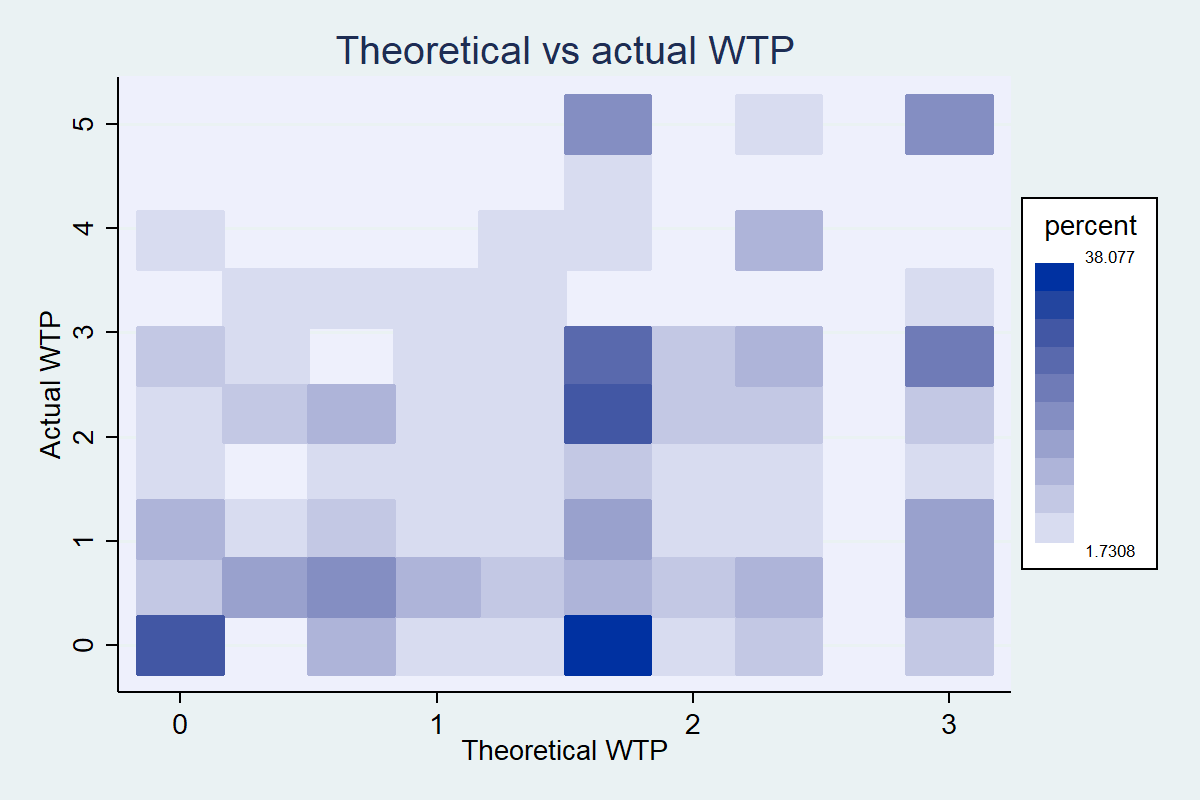
\includegraphics[scale=0.3]{Graphs/WTP_value_heat.png}
\end{figure}

\begin{figure}[H]
\centering
\caption{WTP discrepancy} \label{WTP_discrepancy_fig}

  \centering
  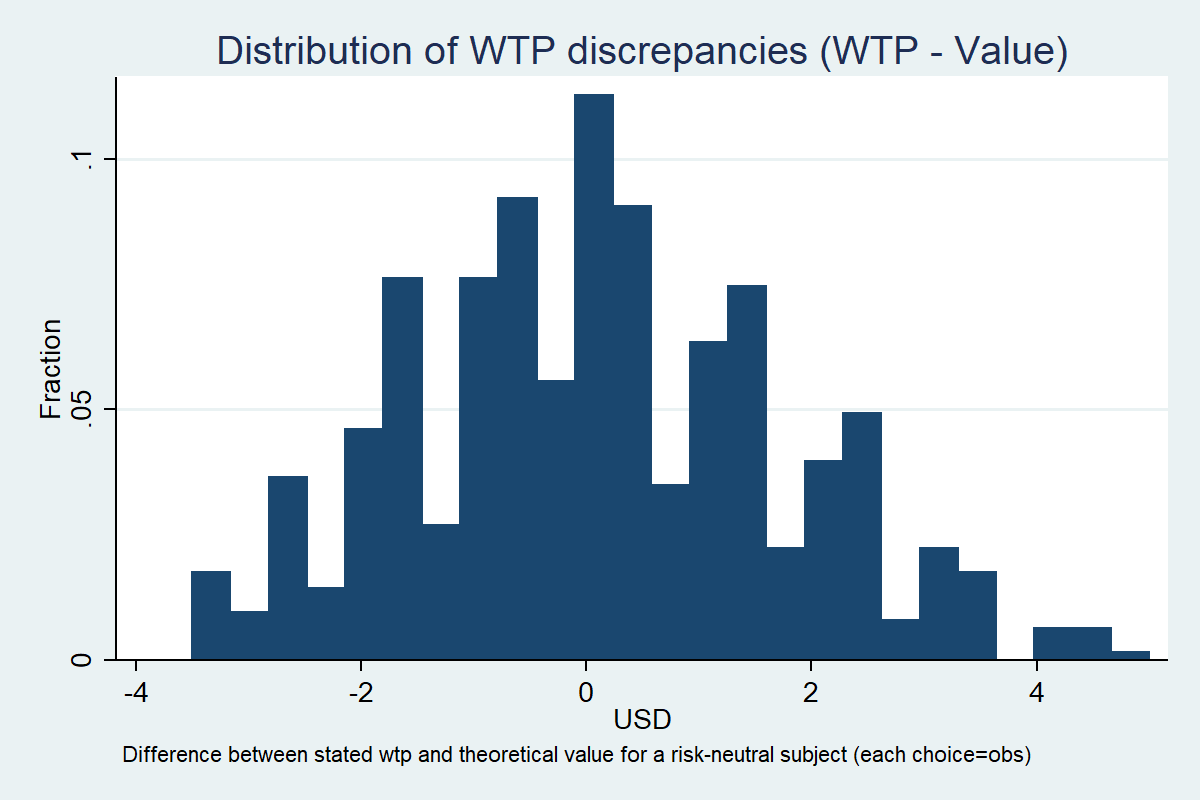
\includegraphics[scale=0.3]{Graphs/hist_WTP_discr1.png}

\end{figure}



\end{document}